\documentclass[12pt, twoside, openright]{report}
\usepackage[utf8]{inputenc}
\usepackage[a4paper, width=150mm, top=25mm, bottom=25mm]{geometry}
% TODO: el espacio en blanco grande de las páginas va a la derecha o a la izquierda?
% TODO: Poner todos los "plugin" en cusriva
% TODO: eliminar todos los RED del documento (buscar ctrl+f)
% TODO: comprobar que los apartados empiezan en la pagina derecha y la izquierda queda en blanco (mirar las reglas de la escuela y todo eso porque parece que solo los capítulos están comenzando así)
% TODO: cambiar nombre de "listings" a "código" o algo así
%%%%%%%%%%%%%%%%%%%%%%%%%%%%%%
%% group functionality %%
% individual functionality %
% ----- "separator"
%%%%%%%%%%%%%%%%%%%%%%%%%%%%%%

%% language %%
\usepackage[spanish]{babel}
\usepackage{csquotes}

% -----

%% images %%
\usepackage{graphicx}

% set default images directory %
\graphicspath{ {images/} }

% include pfs for a3 pages %
\usepackage{pdfpages}

% directory trees %
\usepackage{dirtree}

% table colspan %
\usepackage{multicol}

% table rowspan %
\usepackage{multirow}

% -----

%% links %%
% includes index links %
\usepackage{hyperref}

% -----
% TODO: Volver a poner el header en la primera página de cada seccion
%% headers and footers %%
\usepackage{fancyhdr}
\pagestyle{fancy}

% remove all header and footer content %
\fancyhf{}

% custom header %
\fancyhead[RO,LE]{Winagent - Agente modular para servidores Windows}

% custom footer %
\fancyfoot[RO,LE]{\thepage}

% set top sepparation to 15pt %
\setlength{\headheight}{15pt}

%% redefine emty and plain styles %%
% empty pages are really empty %
\usepackage{emptypage}

% redefine plain stayle to put page numbers in their place in Chapter pages %
\fancypagestyle{plain}{
    \fancyhf{}                              % remove header and footer
    \fancyfoot[RO,LE]{\thepage}             % set position for page numbers
    \renewcommand{\headrulewidth}{0pt}     % remove header line
}

% -----

\usepackage{listings}
\usepackage{lstautogobble}
\usepackage{xcolor}
%New colors defined below
\definecolor{codegreen}{rgb}{0,0.5,0}
\definecolor{codegray}{rgb}{0.5,0.5,0.5}
\definecolor{redstrings}{rgb}{0.64,0.08,0.08}
\definecolor{operatorspurple}{rgb}{0.58,0,0.82}
\definecolor{backcolour}{rgb}{0.95,0.95,0.92}

%Code listing style named "mystyle"
\lstdefinestyle{csharp}{
    language={[Sharp]C},
    autogobble,
    backgroundcolor=\color{backcolour},
    commentstyle=\color{codegreen},
    keywordstyle=\color{blue},
    keywordstyle={[2]\color{operatorspurple}\bf},
    numberstyle=\tiny\color{codegray},
    stringstyle=\color{redstrings},
    basicstyle=\ttfamily\footnotesize,
    breakatwhitespace=false,         
    breaklines=true,                 
    captionpos=b,                    
    keepspaces=true,                 
    numbers=left,                    
    numbersep=5pt,                  
    showspaces=false,                
    showstringspaces=false,
    showtabs=false,                  
    tabsize=4,
    otherkeywords={ JObject },
    morekeywords=[2]{ :, <, >, <<, >>, =, ? }
}

\lstdefinestyle{batch}{
    language={[WinXP]command.com},
    autogobble,
    backgroundcolor=\color{backcolour},
    commentstyle=\color{codegreen},
    keywordstyle=\color{codegray},
    stringstyle=\color{redstrings},
    basicstyle=\ttfamily\footnotesize,
    breakatwhitespace=false,         
    breaklines=true,                 
    captionpos=b,                    
    keepspaces=true,                 
    showspaces=false,                
    showstringspaces=false,
    showtabs=false,                  
    tabsize=4,
    otherkeywords={ 
        --install,
        --uninstall,
        --start,
        --stop,
        --restart,
        --status,
        -Name,
        -BinaryPathName
    }
}

%"mystyle" code listing set
% \lstset{style=csharp}

% -----

%% text options %%
% rename table index %
\renewcommand\listtablename{Índice de tablas}

% set space between paragraphs %
\setlength{\parskip}{1em}

% first paragraph indent %
\usepackage{indentfirst}

% remove "Chapter nº" headings %
\usepackage{titlesec} 
\titleformat{\chapter}{\normalfont\bfseries}{\huge\thechapter}{1em}{\huge}

% -----

%% references %%
% truncate authors if >5
% same order than in the text
\usepackage[maxbibnames=4,sorting=none]{biblatex}
\addbibresource{references.bib}
%% \cite(text)
%% \parencite[see][p10](text)
%% \parencite[compare][](text)
%% \parencite[e.g.][page 300](text)
%% \printbibliography

% -----

%% blank title info %%
% this will generate a blank foil %
% TODO: the title page will be printed separately %
% \title{}
% \date{}

% TODO: eliminar esto, buscar todas las palabras en rojo para comprobarlas (comando \red)
\usepackage{xcolor}
\newcommand{\red}[1]{\textcolor{red}{#1}}

\begin{document}

%% title page %%
% \maketitle

%% indexes %%
\tableofcontents
\listoffigures
\listoftables

%% content %%

% introduction %
\chapter{Introducción}
\label{sec:int}
%haberá que incluír unha introdución ao problema e xustificación do
%traballo realizado. En caso de que o TFG integre ou desenvolva traballos feitos na
%actividade doutras materias da titulación, o/a estudante deberá especificar os devanditos
%traballos e materias nesta sección.*/

La Organización Europea para la Investigación Nuclear, más conocida por sus siglas en francés \textit{CERN}, cuenta con más de treinta mil trabajadores asociados. En sus instalaciones se realiza una gran variedad de actividades diferentes, desde administrativas hasta de planificación e investigación. Entre estas actividades se incluyen siete experimentos en el Large Hadron Collider (\textit{LHC}), el acelerador de partículas más grande del mundo, compuestos por \textit{ATLAS} y \textit{CMS}, donde se utilizan detectores de uso general con el objetivo de abarcar el mayor rango posible de investigación, \textit{ALICE} y \textit{LHCb}, que investigan fenómenos específicos mediante el uso de detectores especializados, \textit{MoEDAL} que está centrado en la búsqueda de una partícula hipotética llamada \textit{the magnetic monopole} mediante el uso de detectores desplegados cerca del \textit{LHCb}, y los más pequeños \textit{TOTEM} y \textit{LHCf}que se centran en el análisis de \textit{fordward particles}, protones o iones pesados que rozan entre sí en lugar de encontrarse frontalmente cuando los haces chocan. \cite{lhc}

Todos estos procesos consumen una gran cantidad de tiempo y recursos, además de las labores de mantenimiento que provocan que el \textit{LHC} esté inoperable por largos períodos de tiempo. Por este motivo son muy importantes las tareas de planificación, preparación y simulación, que permiten que los resultados obtenidos mediante la realización de estos experimentos físicos sean lo más precisos posibles. Para ello es necesario que los servicios utilizados por el personal estén disponibles la mayor parte del tiempo, no sufran degradaciones y que ante cualquier fallo reciban una respuesta inmediata, tanto para evitar, como para resolver una incidencia. Esto incluye, entre otros, la monitorización de fallos en el software, hardware y parcheado de nuevas vulnerabilidades en la seguridad.

En el departamento de \textit{Information Technology} (\textit{IT}) se lleva a cabo la administración de estos servicios y los servidores necesarios para esta tarea. Dentro de este departamento, el grupo \textit{Collaboration, Devices and Applications} (\textit{IT-CDA}) es el encargado de gestionar los servicios de infraestructura, los cuales están directamente relacionados con \textit{Windows}, llegando a gestionar alrededor de 1000 de estos servidores, tanto físicos como virtuales, que incluyen entre otras cosas, los servicios de correo, autenticación, hosting web, virtualización, servidores de licencias, \textit{terminal servers} y servidores personalizados para cualquier departamento, grupo o experimento que lo requiera. \cite{infraservicios,infrawindows}

Actualmente la monitorización de estos servidores es realizada mediante \textit{SNMP} o \textit{scripts} que se ejecutan periódicamente, tomando información tanto del estado del hardware como del software, y filtrando algunos de los \textit{logs} que deben ser analizados. Esta información filtrada es enviada mediante correo electrónico a la persona responsable del área a la que pertenece la información, quien debe revisarla manualmente para descubrir cualquier incidencia ocurrida.

Un ejemplo de esto es la monitorización de las unidades de almacenamiento colocadas en la máquinas físicas. Los discos duros están configurados como \textit{RAID 1} (ver anexo \ref{anx:raid1}), lo que permite tener cierto nivel de resistencia a fallos, sin embargo, ante el mal funcionamiento de uno de los dispositivos, este tiene que ser reemplazado inmediatamente, ya que en caso de fallar el siguiente se perdería toda la información.

El proceso de detección de fallos en los discos duros comienza con \textit{scripts} que filtran diariamente los \textit{logs} generados por los sistemas actuales de monitorización y eventos del sistema (\textit{Event Logs}), con palabras como ``\textit{Fail}'', ``\textit{Failure}'' o ``\textit{Error}'', en el anexo \ref{anx:hw-info} se muestra un fragmento de uno de estos filtros. Una vez la información es recibida por el responsable, debe proceder a revisarla y, en caso de encontrar algún fallo, este deberá crear un \textit{ticket} de soporte para garantizar el remplazo del disco.

Debido a que el procedimiento mencionado representa una gran cantidad de tiempo y esfuerzo para cada una de las personas que deban desempeñar dichas tareas, surge el planteamiento base para el desarrollo de esta aplicación, la creación de una herramienta que sea capaz de englobar estos procesos de recopilación de información y servirla a diferentes sistemas de monitorización donde sea requerida para tomar las medidas oportunas. Además, crear esta aplicación personalizada, frente a otras soluciones como las basadas en \textit{SNMP}, permite abarcar de forma sencilla información requerida específicamente por la organización, por ejemplo, la información referente a las actualizaciones de \textit{Windows}.

El desarrollo de este proyecto es llevado a cabo en paralelo con \textit{CHOPIN}, un sistema de monitorización desarrollado por \textit{Marta Pacuszka}, el cual es el encargado de gestionar toda la información recibida desde \textit{Winagent} y presentarla al usuario utilizando una interfaz amigable, donde se puedan distinguir claramente las acciones necesarias en cada uno de los servidores.

Cabe mencionar que este proyecto, pese a ser una solución a un problema interno del \textit{CERN}, no está limitado a sus requisitos, es de código abierto y puede ser implementado en cualquier institución que cumpla con las condiciones necesarias para su instalación, además de que permite, debido a su carácter modular, la adición de funcionalidades para obtener y enviar información de casos de uso particulares.


% presentar o problema que se vai tratar, incluír o obxectivo principal e os
% específicos, de ser o caso, do traballo presentado, indicando o alcance para cada un deles.

\section{Objetivos} \label{sec:obj}
    En esta sección se especifican los objetivos que persigue el proyecto presentado. Se incluyen tanto los objetivos principales, donde se describe una solución general que se desea obtener del proceso de desarrollo, como los objetivos específicos donde se detalla qué es lo que se busca en cada una de las partes del sistema.

    \subsection{Objetivo principal}
        El objetivo principal que persigue este proyecto es la creación de una herramienta modular que permita, de forma automatizada, obtener periódicamente información de los sistemas y funcionalidades que deban ser monitorizados en cada uno de los servidores \textit{Windows} y servirla a diferentes sistemas de monitorización enfocados en el usuario, que podrán ser utilizados para tomar las medidas oportunas.
        
        Esto representa un gran avance para la situación actual de la monitorización, donde la mayoría de las acciones son tomadas en función de comprobaciones realizadas manualmente o mediante el uso de \textit{scripts} que, a pesar de facilitar la obtención de datos relevantes, no están organizados de forma centralizada.
        
        La implantación de este nuevo sistema de monitorización se traduce en un ahorro de tiempo y esfuerzo por parte de los administradores de los servidores. Además, proveer una interfaz intuitiva con un panel donde los fallos, actualizaciones pendientes, amenazas, etc. sean fácilmente identificables, permitirá prevenir errores y aplicar las actualizaciones necesarias lo antes posible.
        
    \subsection{Objetivos específicos}
        \begin{itemize}
            \item \textbf{Sistema modular:} \\
                El sistema estará compuesto por un agente y varios \textit{plugins}, que será capaz de gestionar y comunicar, además de proveerlos con las configuraciones necesarias para que realicen funcionalidades específicas.
                
            \item \textbf{Plugins de entrada:} \\
                La información del sistema será recopilada mediante el uso de \textit{plugins de entrada}, los cuales no tendrán un funcionamiento autónomo y estarán centrados en una información específica.
                
            \item \textbf{Plugins de salida:} \\
                Los datos recibidos desde los \textit{plugins de entrada} serán utilizados por los \textit{plugins de salida}, los cuales enviarán la información a los sistemas de gestión de información o la presentarán directamente al usuario.
                
            \item \textbf{Sistema de planificación:} \\
                Los \textit{plugins} se ejecutarán periódicamente a través del \textit{agente}. De esta forma se controlará tanto el orden como la frecuencia de obtención y transmisión de la información.
                  
            \item \textbf{Captura de eventos del sistema:} \\
                El \textit{agente} podrá ser suscrito a los \textit{logs} de eventos del sistema. La información generada en estos \textit{logs} en tiempo real será utilizada por los \textit{plugins de salida} especificados.
            
            \item \textbf{Actualizador automático:} \\
                Tanto el \textit{agente} como los \textit{plugins} deberán ser actualizados automáticamente siempre que haya una nueva versión disponible. El \textit{sistema de planificación} se encargará de que este proceso se realice de forma regular.
                
            \item \textbf{Archivo de configuración:} \\
                Se utilizará un archivo de configuración donde se especifiquen las opciones con las que serán ejecutadas todas las funcionalidades del sistema. Esto incluye tanto el actualizador como los \textit{plugins}, sus períodos de ejecución, y vinculaciones.
                
            \item \textbf{Servicio:} \\
                El sistema podrá ser iniciado como un \textit{Servicio} que se mantenga en ejecución permanentemente en segundo plano. De esta forma podrá llevar a cabo todas las tareas configuradas sin la intervención del usuario. Además, iniciará automáticamente con el arranque del sistema operativo.
                
            \item \textbf{Interfaz de línea de comandos (\textit{CLI}):} \\
                Mediante el uso de una consola de comandos se podrá controlar la instalación y estado del \textit{servicio}. Además, se podrá consultar la información del servidor utilizando un archivo de configuración o especificando manualmente los \textit{plugins} que se desea ejecutar junto con las opciones necesarias para ello. La impresión por pantalla de la información será llevada a cabo por un \textit{plugin de salida} específico, el cual será la salida predeterminada para la \textit{CLI}.
        \end{itemize}


\section{Resumen de la solución propuesta} \label{sec:sol}
% indicarase a solución aportada para o problema
% presentado. Deberase incluír aquí a metodoloxía empregada.

    Tras una fase de investigación para determinar las bases del proyecto, limitaciones e información que es necesario recopilar en los servidores, se ha realizado una comparativa entre los principales lenguajes de programación creando una aplicación con funcionalidades mínimas (acceder a librerías del sistema). Estas actividades han permitido tomar las siguientes decisiones.
    
    Se creará un \textit{agente modular} utilizando el lenguaje de programación \textit{CSharp}, más concretamente \textit{.NET Framework} debido a la alta compatibilidad que brinda con las librerías de \textit{Windows}. Esto permitirá utilizar los mecanismos que proporciona el sistema operativo para obtener información propia.
    
    Los \textit{plugins} serán creados como librerías externas que podrán ser cargadas por el \textit{agente} en caso de estar en una carpeta específica durante su ejecución. La comunicación entre los \textit{plugins de entrada} y \textit{plugins de salida} se realizará mediante \textit{cadenas de texto} en formato \textit{JSON}, y ambos deberán recibir los parámetros necesarios en este mismo formato.
    
    Se utilizarán sistemas de control de versiones y se creará un repositorio para cada uno de los componentes, configurando mecanismos de \textit{integración continua} que permitan automatizar los procesos de compilación y publicación de nuevas versiones. Las publicaciones creadas proveerán con la información necesaria al sistema de actualización automática.
    
    El mecanismo de actualización automática se encargará de mantener actualizado al agente, cada uno de los \textit{plugins} y a sí mismo. Para esto, comprobará periódicamente la última versión estable disponible, si esta es superior a la que está instalada actualmente, la reemplazará. Dado que mientras los componentes de la aplicación están siendo utilizados no pueden ser modificados, el sistema de actualización será creado como una aplicación independiente encargada de terminar el proceso del agente, llevar a cabo la actualización, e iniciarlo una vez finalizado este.
    
    Los ajustes de la aplicación se establecerán en formato \textit{JSON}, separando las configuraciones en tres bloques: el actualizador, los eventos del sistema y los \textit{plugins}. En los dos últimos, la configuración de entrada recogerá los detalles de la configuración de salida, que incluirá, además de sus propias opciones, la frecuencia con la que se obtendrán los datos para transmitirlos por esa vía.
    
    En la figura \ref{fig:proposed-solution-diagram} se puede apreciar un diagrama resumen de la solución propuesta para la realización de este proyecto.
    
    \begin{figure}[h!]
    \centering
        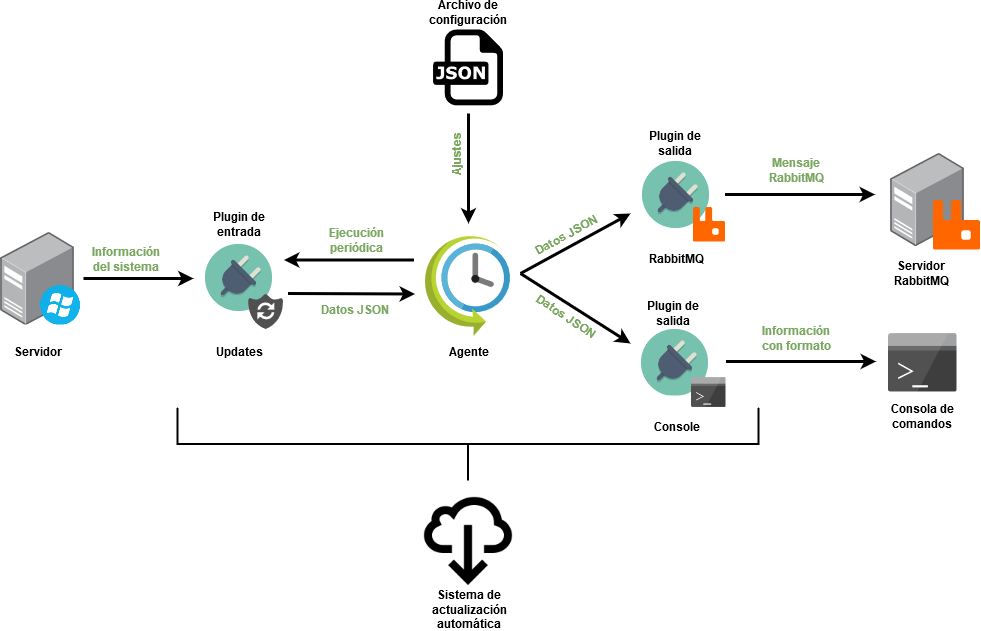
\includegraphics[scale=0.5]{diagrama-solucion-propuesta.png}
        \caption{Resumen de la solución propuesta}
        \label{fig:proposed-solution-diagram}
    \end{figure}
    
    Este proyecto parte de objetivos bien definidos y cierto nivel de detalle, sin embargo, una gran parte del sistema a desarrollar depende en su totalidad de librerías tanto de \textit{Windows} como de terceros. Esto es una limitación, y hace que la planificación inicial pueda variar debido a incompatibilidades entre ellas. Debido a esto se ha concluido que lo más adecuado sería el uso de un método ágil de desarrollo de software, en concreto \textit{SCRUM}, que está más enfocado a la administración del desarrollo iterativo. \textit{SCRUM} consta de tres fases:
        
    \begin{itemize}
        \item Planificación de un \textit{boceto}, donde se establecen los objetivos generales del proyecto y el diseño de la arquitectura del software.
        
        \item Una serie de ciclos \textit{sprint}, donde cada ciclo desarrolla un incremento del sistema.
        
        \item \textit{Cierre} del proyecto, fase en la cual se completa la documentación requerida como ayudas y manuales de usuario.
    \end{itemize}

    \textit{SCRUM} permite que el producto se desglose en piezas comprensibles de forma individual y que son desarrolladas de forma iterativa, recibiendo retroalimentación del usuario con cada entrega y realizando cambios en consecuencia. Para llevar a cabo el desarrollo utilizando este método, es necesario ocupar los roles imprescindibles para su funcionamiento.

    \begin{itemize}
        \item \textbf{Equipo de desarrollo:} Equipo responsable de llevar a cabo el desarrollo del sistema. Este rol estará compuesto únicamente por el alumno.
        
        \item \textbf{Cliente:} Encargado de definir los requisitos, utilizar las versiones resultantes de cada \textit{sprint} y aportar retroalimentación para la mejora del sistema. Este rol será llevado a cabo por el supervisor del proyecto.
        
        \item \textbf{Maestro de SCRUM:} Encargado de rastrear el trabajo que queda por hacer, tomar decisiones, medir el avance en función de la planificación inicial y mantener la comunicación con el cliente. Este rol será adoptado por el supervisor del proyecto.
    \end{itemize}
    
    


% description %
\chapter{Descripción del trabajo}

\red{En esta sección se presenta una descripción detallada de todo lo relacionado con el desarrollo de del proyecto, se abarcan los temas relacionados con la Ingeniería de Software, así como los procesos seguidos y tecnologías utilizadas. Permite conocer los procesos seguidos desde la planificación planteada inicialmente hasta la finalización del proyecto, incluyendo las desviaciones ocurridas}

\section{Planificación y seguimiento} \label{sec:plan}
% deberase incluír un diagrama de Gantt que amose tanto
% a planificación do traballo, coa súa distribución de fases e tarefas, e a súa comparación cos
% datos reais obtidos tras o desenvolvemento do traballo.
    
    Como se expone en el apartado \ref{sec:sol}, la metodología de desarrollo elegida para este proyecto es \textit{SCRUM}.  En este apartado se explica cómo se llevan a cabo todas sus fases, las historias de usuario y tareas incluidas en cada una de ellas, y las desviaciones ocurridas.
    
    \subsection{Historias de usuario}
    
        A continuación se presentan las historias de usuario planteadas inicialmente:
    
        \begin{tabular}{ll}
            \textbf{Como}   & \red{desarrollador}                                                   \\
            
            \textbf{Quiero} & que el sistema sea modular                                            \\
            
            \textbf{Para}   & incorporar nuevas funcionalidades sin modificar el sistema            \\
        \end{tabular}
    
        \begin{tabular}{ll}
            \textbf{Como}   & administrador                                                         \\
            
            \textbf{Quiero} & ejecutar la aplicación como un servicio                               \\
            
            \textbf{Para}   & que se mantenga permanentemente en ejecución                          \\
        \end{tabular}
        
        \begin{tabular}{ll}
            \textbf{Como}   & administrador                                                         \\
            
            \textbf{Quiero} & ejecutar la aplicación desde la consola de comandos                   \\
            
            \textbf{Para}   & realizar ejecuciones manuales                                         \\
        \end{tabular}
        
        \begin{tabular}{ll}
            \textbf{Como}   & administrador                                                         \\
            
            \textbf{Quiero} & especificar la configuración en un archivo                            \\
            
            \textbf{Para}   & desplegar el sistema fácilmente en varios servidores                  \\
        \end{tabular}
        
        \begin{tabular}{ll}
            \textbf{Como}   & administrador                                                         \\
            
            \textbf{Quiero} & capturar eventos del sistema en tiempo real                           \\
            
            \textbf{Para}   & detectar errores en el servidor lo antes posible                      \\
        \end{tabular}
        
        \begin{tabular}{ll}
            \textbf{Como}   & administrador                                                         \\
            
            \textbf{Quiero} & que la aplicación se actualice automáticamente                        \\
            
            \textbf{Para}   & tener siempre la aplicación actualizada en todos los servidores       \\
        \end{tabular}
        
        \begin{tabular}{ll}
            \textbf{Como}   & administrador                                                         \\
            
            \textbf{Quiero} & obtener información de las actualizaciones del Sistema Operativo      \\
            
            \textbf{Para}   & controlar los servidores desactualizados                              \\
        \end{tabular}
        
        \begin{tabular}{ll}
            \textbf{Como}   & administrador                                                         \\
            
            \textbf{Quiero} & tener un sistema de latidos                                           \\
            
            \textbf{Para}   & saber cuando un servidor ha fallado                                   \\
        \end{tabular}
        
        \begin{tabular}{ll}
            \textbf{Como}   & administrador                                                         \\
            
            \textbf{Quiero} & que la información sea mostrada en consola                            \\
            
            \textbf{Para}   & depurar error con comprobaciones manuales                             \\
        \end{tabular}
        
        \begin{tabular}{ll}
            \textbf{Como}   & administrador                                                         \\
            
            \textbf{Quiero} & que la información se envíe a un servidor RabbitMQ                    \\
            
            \textbf{Para}   & poder consumirla con otros sistemas                                   \\
        \end{tabular}
        
    \subsection{Planificación inicial}
        Como se muestra en la tabla \ref{tab:fases-planif}, el desarrollo del sistema se llevará a cabo durante nueve fases, entre las cuales se incluyen cinco \textit{sprints} de implementación y la elaboración de la documentación, que incluye la fase de cierre, fundamental en \textit{SCRUM}
            
        \begin{table}[h!]             
            \centering                  
                \resizebox{\textwidth}{!}{   
                    \begin{tabular}{|l|c|c|}
                        \hline
                        \multirow{2}{*}{\textbf{Fase}}      & \multicolumn{2}{|c|}{\textbf{Estimación temporal}}    \\
                        \cline{2-3}
                                                            &   Días                &   Horas                       \\
                        \hline
                        Spike                               &   4                   &   12                          \\
                        Pruebas con diferentes lenguajes    &   4                   &   12                          \\
                        Boceto                              &   2                   &   6                           \\
                        Sprint 1                            &   15                  &   45                          \\
                        Sprint 2                            &   15                  &   45                          \\
                        Sprint 3                            &   15                  &   45                          \\
                        Sprint 4                            &   15                  &   45                          \\
                        Sprint 5                            &   10                  &   30                          \\
                        \hline
                        \hline
                        Documentación                       &   80                  &   240                         \\
                        \hline                  
                        \hline                  
                        \textbf{Total}                      &   \textbf{80}         &   \textbf{240}                \\
                        \hline
                    \end{tabular}
                }
            \caption{Planificación de las fases}
            \label{tab:fases-planif}
        \end{table}
        
        En las imágenes \ref{fig:gantt-initial-tasks} y \ref{fig:gantt-initial-diagram} se puede apreciar la planificación en el tiempo de las nueve fases antes mencionadas.
        
        \begin{figure}[h!]
        \centering
            \frame{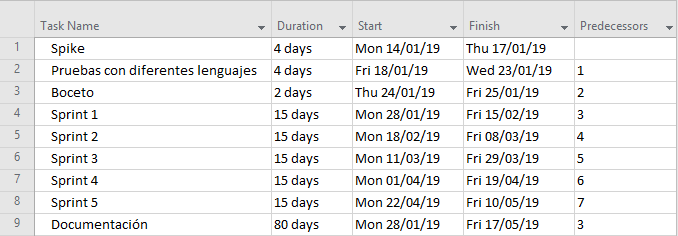
\includegraphics[scale=0.7]{planificacion-inicial-tareas.png}}
            \caption{Planificación de las fases del proyecto}
            \label{fig:gantt-initial-tasks}
        \end{figure}
        
        \begin{figure}[h!]
        \centering
            \frame{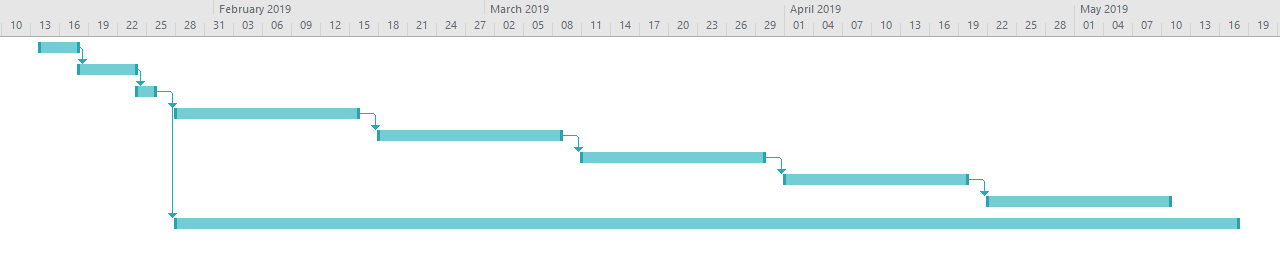
\includegraphics[scale=0.44]{planificacion-inicial-diagrama.png}}
            \caption{Diagrama de Gantt de la planificación inicial}
            \label{fig:gantt-initial-diagram}
        \end{figure}
        
    \subsection{Seguimiento del proyecto}
        
        Las imágenes \ref{fig:gantt-followup-tasks} y \ref{fig:gantt-followup-diagram} muestran la planificación detallada de las tareas del proyecto. Es importante destacar que debido a actividades no relacionadas con la aplicación, o actividades que aunque sean relacionadas con la aplicación, no son incluidas en este proyecto, el proceso de desarrollo se ha visto afectado en ciertos momentos. \red{poner cómo lo ha afectado?}
        
        \begin{figure}[h!]
        \centering
            \frame{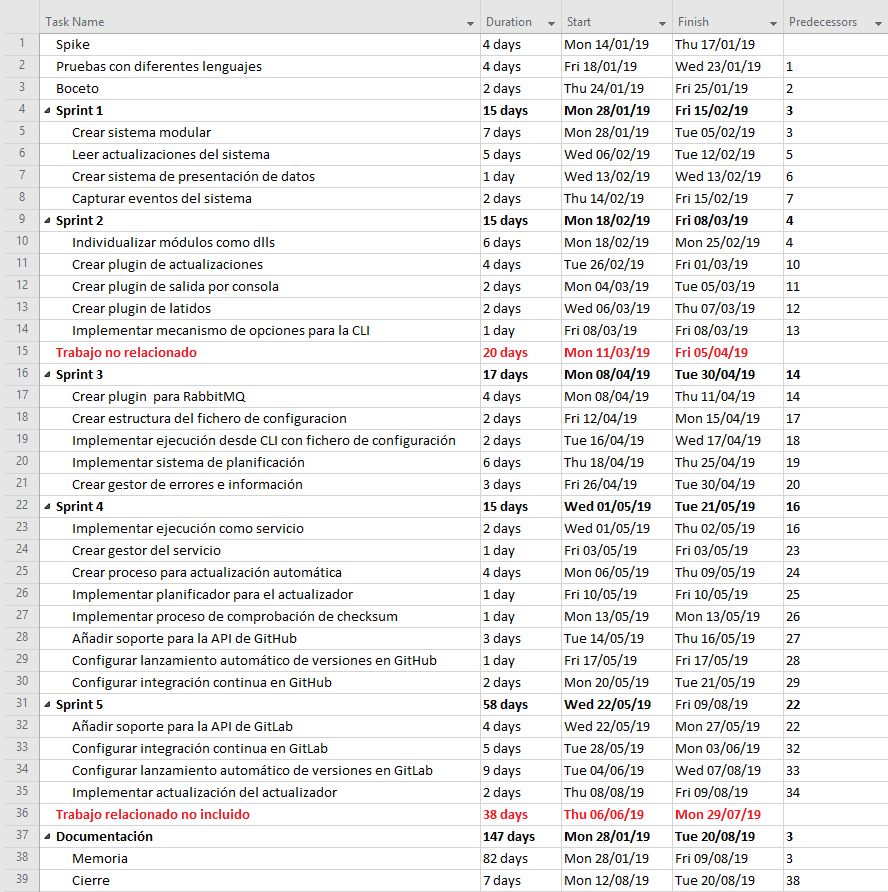
\includegraphics[scale=0.6]{seguimiento-tareas.png}}
            \caption{Planificación de las tareas del proyecto}
            \label{fig:gantt-followup-tasks}
        \end{figure}
    
        \begin{figure}[h!]
        \centering
            \frame{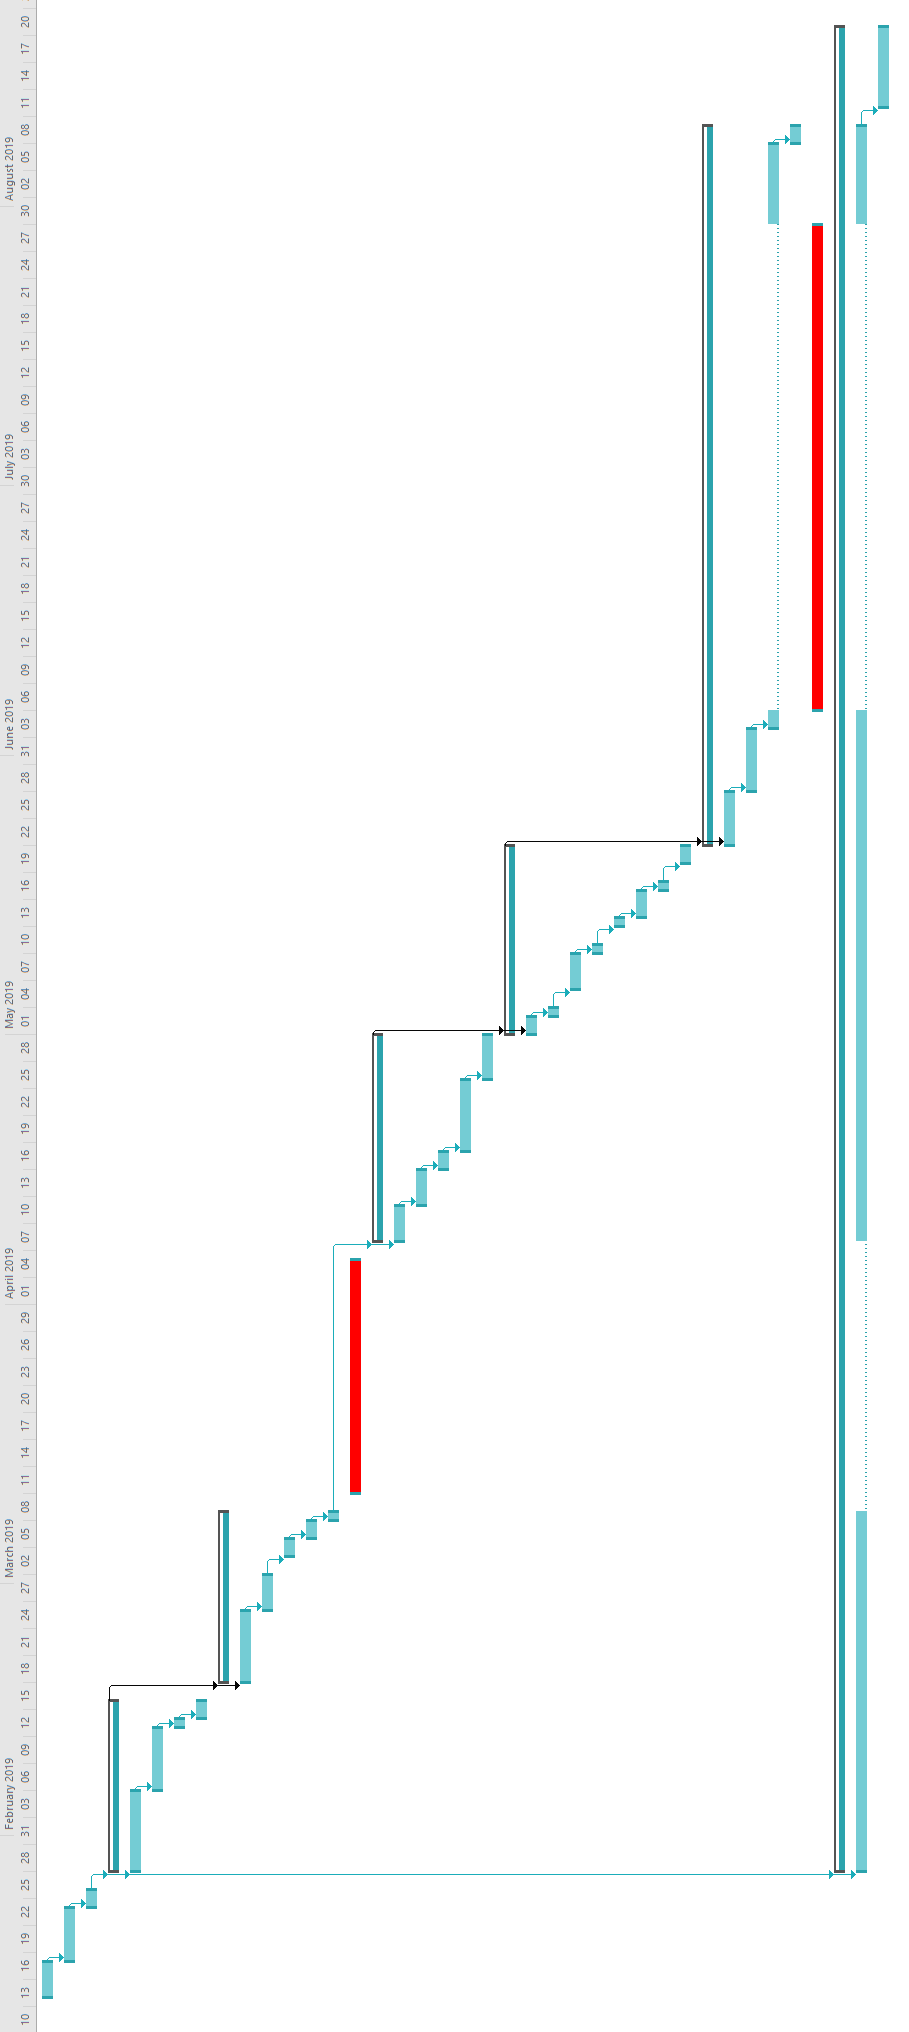
\includegraphics[scale=0.44]{seguimiento-diagrama.png}}
            \caption{Diagrama de Gantt de la planificación de tareas}
            \label{fig:gantt-followup-diagram}
        \end{figure}
\cleardoublepage
\section{Arquitectura y tecnologías} \label{sec:arq}
% explicarase a arquitectura empregada para alcanzar os obxectivos propostos.

    \subsection{Arquitectura del sistema}

        Se entiende que dada la variedad y versatilidad del sistema, no existe una arquitectura que pueda definirlo en su totalidad, ya que cada uno de los plugins tiene una forma de desarrollo y método de comunicación que depende directamente de su funcionalidad. Sin embargo, se puede decir que la arquitectura general del sistema está enfocada en un modelo \textit{Basado en componentes}.
        
        Este modelo de desarrollo de software enfatiza la descomposición del diseño en componentes funcionales o lógicos que se comuniquen mediante interfaces bien definidas. Esto permite alcanzar un mayor nivel de abstracción, ya que no se enfoca en las características específicas de cada componentes sino en el sistema en sí, y en la forma en que estos componentes son integrados.
        
        El \textit{desarrollo basado en componentes} ofrece algunas ventajas claras en este caso:
        \begin{itemize}
            \item \textbf{Facilidad de instalación y mantenibilidad} \\
            Tanto el software principal como los componentes son fácilmente reemplazables por nuevas versiones sin impacto en el resto del sistema.
            
            \item \textbf{Facilidad de desarrollo} \\
            Los componentes implementan interfaces bien definidas que proveen funcionalidades específicas, por lo que pueden ser desarrollados sin impactar otras partes del sistema.
            
            \item \textbf{Reusabilidad} \\
            Al definir componentes individuales, estos pueden ser reutilizados por diferentes aplicaciones y sistemas con características similares.
            
            \item \textbf{Aumento exponencial de funcionalidades} \\
            El desarrollo de componentes que interactúan entre sí permite que las nuevas funcionalidades puedan ser combinadas con las ya existentes, lo que posibilita satisfacer múltiples casos de uso con cada nueva integración.
        \end{itemize}

        \subsubsection{Componentes del sistema}
            En este apartado se detallan las diferentes partes que componen el sistema, así como la forma en la que se comunican entre ellas. En la figura \ref{fig:diagrama-de-componentes} se muestra un diagrama con los principales componentes, las interfaces de comunicación y los requisitos de cada uno de ellos.

            \begin{figure}[h!]
            \centering
                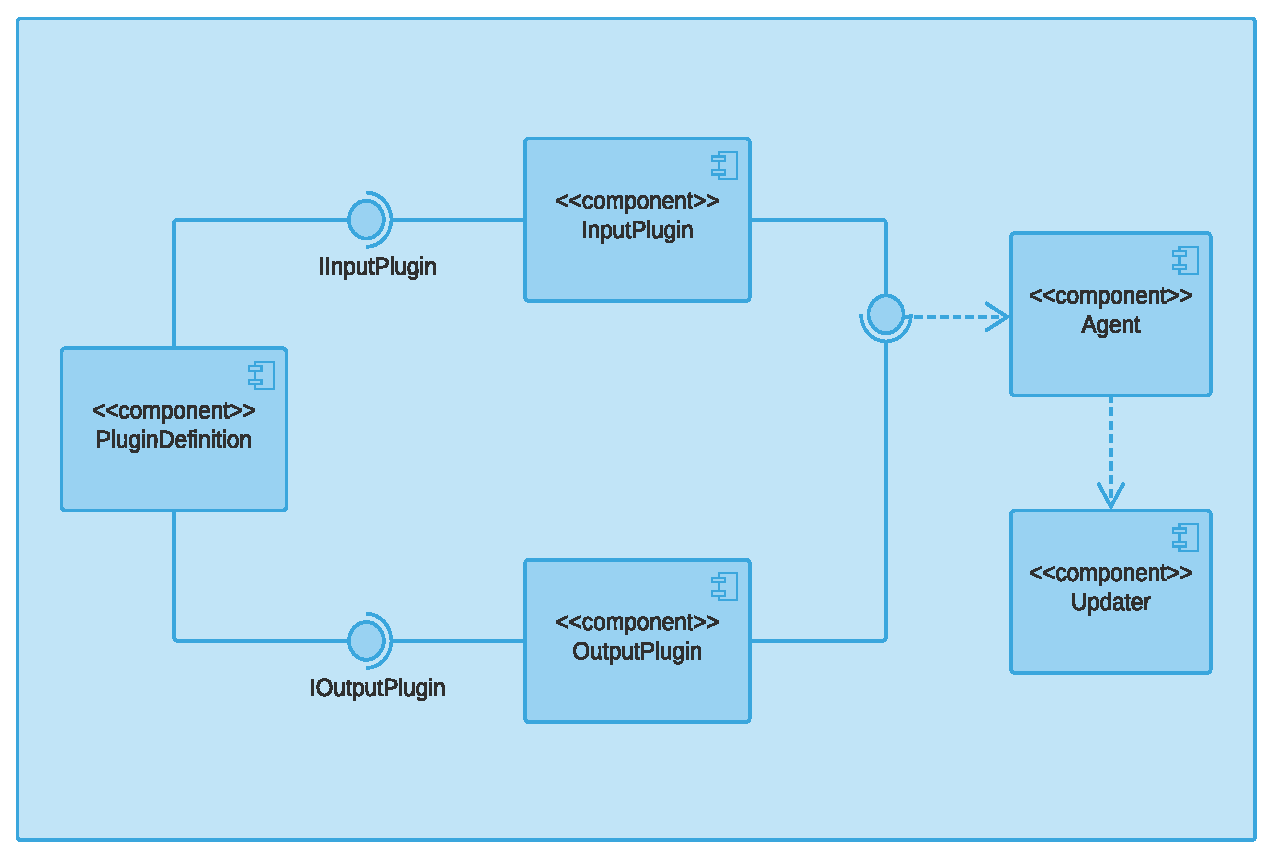
\includegraphics[scale=0.7]{diagrama-de-componentes.eps}
                \caption{Diagrama de componentes}
                \label{fig:diagrama-de-componentes}
            \end{figure}

        \subsubsection{Agente}
            El agente es el encargado de llevar a cabo la ejecución de los \textit{plugins} con las opciones y configuraciones especificadas por el usuario, ya sea a través la línea de comandos o de un archivo de configuración. Además, será el responsable de ejecutar el proceso de actualización automática siempre que este haya sido configurado previamente. Está compuesto por un conjunto de clases, cada una de ellas realiza una tarea específica que le permite funcionar como un todo. En la figura \ref{fig:diagrama-de-arquitectura-winagent} se puede ver la estructura del agente.
            
            \begin{figure}[h!]
            \centering
                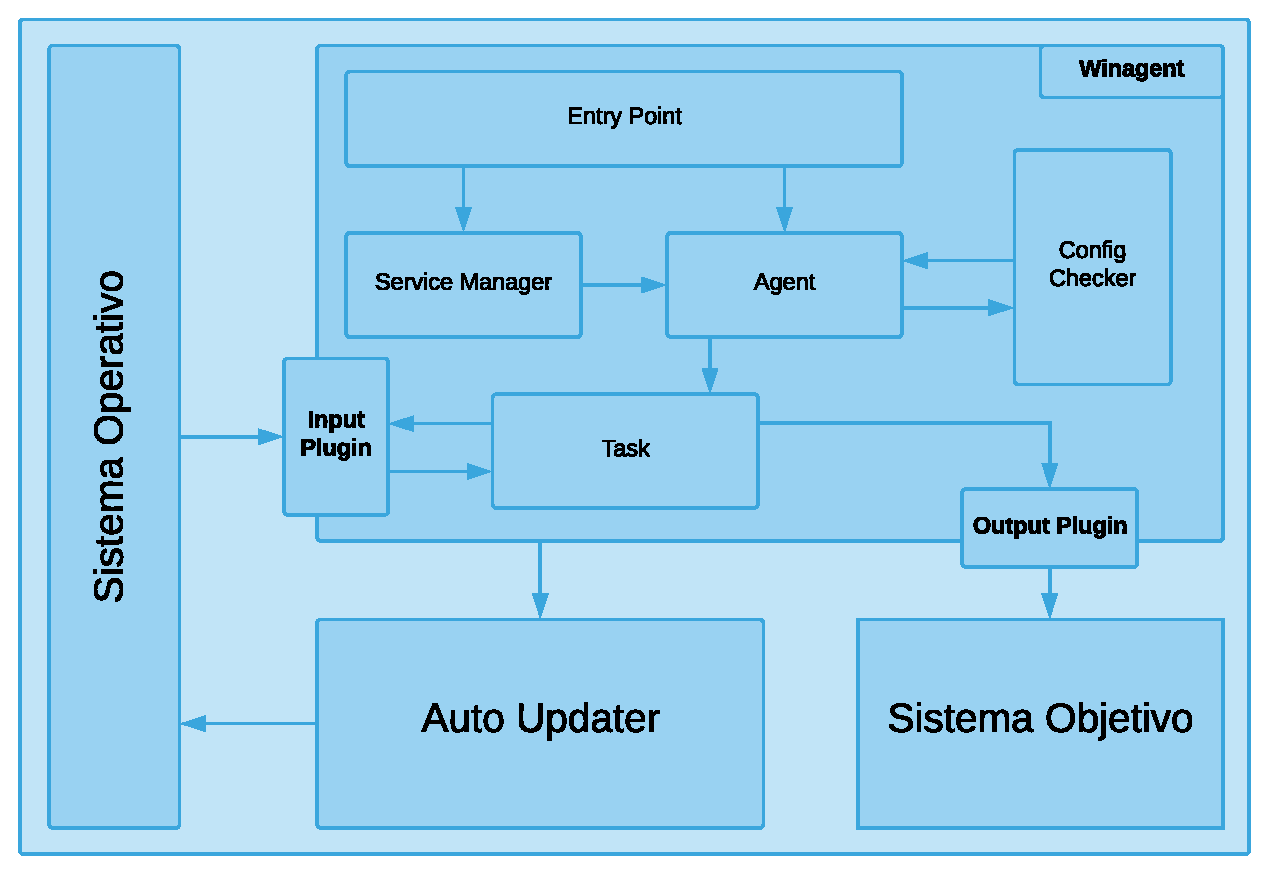
\includegraphics[scale=0.7]{diagrama-de-arquitectura-winagent.eps}
                \caption{Diagrama de arquitectura del sistema}
                \label{fig:diagrama-de-arquitectura-winagent}
            \end{figure}

            Las clases que componen el agente están separadas por su funcionalidad, interactúan entre sí y pueden ser utilizadas durante la ejecución o no, de acuerdo a las opciones y configuración establecidas. Entre las clases se pueden encontrar las encargadas de la inicialización del agente, las que gestionan el agente y sus configuraciones, y las que procesan y transmiten la información entre \textit{plugins}.

            \begin{enumerate}
                \item Sistema de inicialización
                    \begin{itemize}
                        \item \textbf{Punto de entrada} \\
                        Sistema encargado de la inicialización del programa, determina si debe ser iniciado desde consola o como servicio en función del entorno desde el que sea ejecutado, y utiliza las opciones que le sean indicadas por el \textit{Analizador de comandos}.
                            
                        \item \textbf{Gestor de servicios} \\ 
                        Encargado de llevar a cabo la gestión del agente cuando se especifican opciones de control de servicio. Esto incluye instalación, desinstalación, ejecución y detención.
                            
                        \item \textbf{Analizador de comandos} \\ 
                        Es el sistema encargado de analizar sintácticamente las opciones introducidas por el usuario, las cuales varían para ejecuciones como servicio, consola con archivo de configuración predefinido y consola con opciones introducidas mediante linea de comandos.
                    \end{itemize}
                \item Planificador
                    \begin{itemize}
                        \item \textbf{Gestor de configuración} \\ 
                        Encargado de leer el archivo de configuración y proveer al \textit{Sistema de planificación} con la información definida previamente por el usuario.
                        
                        \item \textbf{Sistema de planificación} \\
                        En caso de que la orden sea ejecutada correctamente en el \textit{Sistema de funciones de configuración}, se envía un mensaje de confirmación específico dependiendo de la orden que haya sido recibida y procesada.
                    \end{itemize}
                \item Transmisor de información
                    \begin{itemize}
                        \item \textbf{Plugins de entrada} \\ 
                        Son los plugins encargados de recopilar información del sistema mediante el uso de librerías \textit{.NET}. Sirven esta información a los \textit{Plugins de salida}
                            
                        \item \textbf{Plugins de salida} \\
                        Son los plugins encargados de hacer llegar a la información recopilada por los \textit{Plugins de entrada} a los \textit{sistemas objetivos}. Dependiendo de la finalidad para la que hayan sido creados pueden utilizar diferentes métodos, desde mostrar datos por pantalla hasta enviarlos a un servidor remoto.
                        
                        \item \textbf{Tarea} \\
                        Es la funcionalidad que conecta los \textit{Plugins de entrada} con los \textit{Plugins de salida}, permitiendo que el primero reciba todos los parámetros configurados y agrupándolos como un único elemento capaz de ser configurado en el planificador.
                        
                    \end{itemize}
            \end{enumerate}

        \subsubsection{Actualizador automático}
            El sistema de actualización automática es el encargado de comprobar de forma periódica si las versiones instaladas son las últimas disponibles, esto incluye tanto el \textit{Agente} como los \textit{plugins} y el propio actualizador.
            
            La ejecución de este sistema se realiza en un proceso separado, de forma
            funciona como un script
             itera por todos los componentes del sistema
        
            

            \begin{figure}[h!]
            \centering
                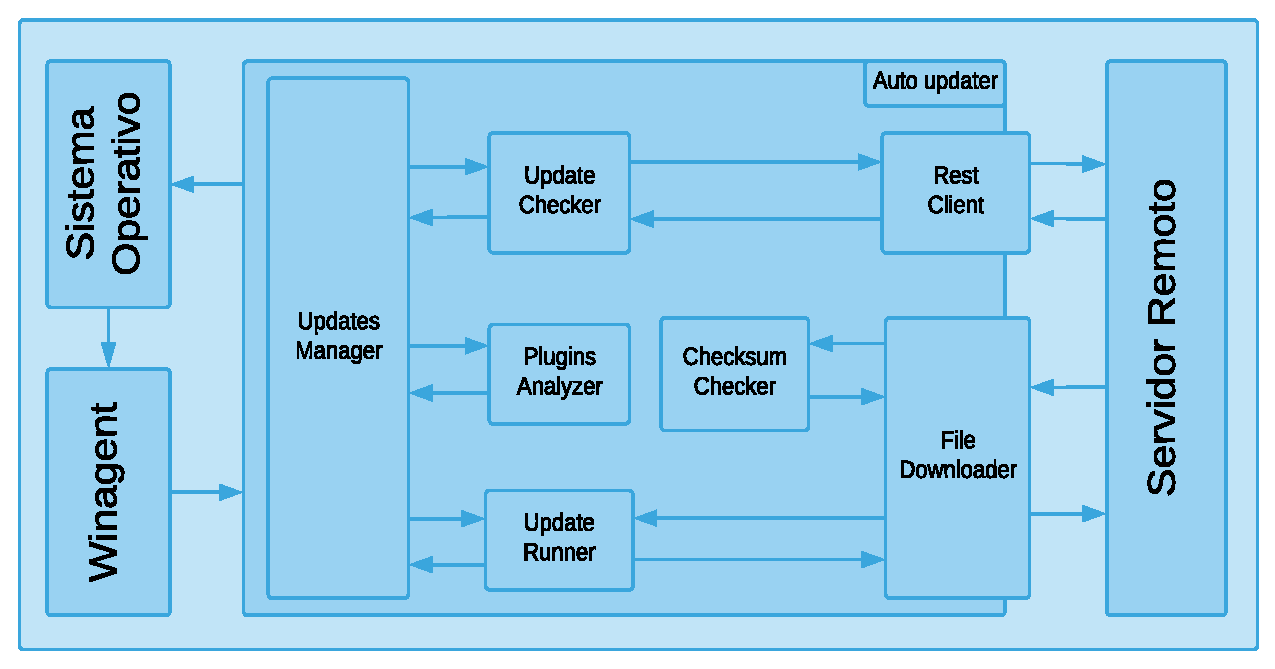
\includegraphics[scale=0.7]{diagrama-de-arquitectura-updater.eps}
                \caption{Diagrama de arquitectura del actualizador}
                \label{fig:client_diagram}
            \end{figure}
            
            

    \red{EXPLICAR LA FUNCIONALIDAD DE LOS COMPONENTES DEL ACTUALIZADOR}
            
            
    % TODO: Estructure del "paquete" datos enviados

    \subsection{Tecnologías e integración de productos de terceros}
    % describiranse adecuadamente as tecnoloxías utilizadas para o desenvolvemento do traballo, así coma os diversos productos que non son da autoría do/da estudante, xustificando a súa utilización.
        \subsubsection{Microsoft Windows}
            Microsoft Windows es el nombre que recibe la familia de distribuciones basada en MS-DOS o Windows NT, desarrollada y comercializada por Microsoft Corporation. Estas estas distribuciones están disponibles para múltiples arquitecturas tales como \textit{x86}, \textit{x86-64} o \textit{ARM}, y hay opciones tanto para dispositivos de uso cotidiano como para servidores y sistemas de alta demanda. \cite{wikiwindows}
            
            Microsoft Windows, además, permite el uso de servicios \cite{wikiservicios}, programas que se ejecutan en segundo plano, proveyendo funcionalidades de forma transparente sin la necesidad de intervención por parte del usuario. Esta funcionalidad es perfecta para la utilización de un software que actúe como agente y se mantenga en ejecución permanentemente, proveyendo datos del equipo donde está instalado.
            
            \begin{itemize}
                \item \textbf{Windows 10} \\
                Dadas las similitudes de los sistemas \textit{Windows}, esta distribución pensada para la utilización de usuarios en entornos personales y laborales es la utilizada para el desarrollo del sistema que se propone. Permite llevar a cabo la creación del sistema de forma cómoda, sin necesidad de construir el entorno de desarrollo en un servidor administrado de forma remota.
                
                \item \textbf{Windows 2012 R2} \\
                Es la distribución instalada en la mayoría de servidores \textit{Windows} del CERN y sobre los que se desea utilizar el sistema que se desarrolla. Es utilizada para realizar pruebas periódicas que garanticen la compatibilidad con la plataforma de desarrollo; también se utiliza par llevar a cabo los procesos de construcción y publicación gestionados por \textit{gitlab-ci} en cada versión lanzada.
                
            \end{itemize}

        \subsubsection{Lenguaje C\#}
            Es un lenguaje de programación orientado a objetos diseñado y estandarizado por Microsoft como parte de \textit{.NET}, con el objetivo de permitir el desarrollo de aplicaciones y sistemas que fueran independientes de la arquitectura física y del sistema operativo sobre el que se ejecutaran. Es actualmente el lenguaje de programación más eficiente a la hora de trabajar con librerías de Windows por las facilidades que brinda para este tipo de desarrollos. \cite{csharp}

            \begin{itemize}
                \item \textbf{.NET Framework} \\
                Es una versión solo para \textit{Windows} de \textit{.NET}, la cual brinda interoperabilidad y cuenta con una gran librería de clases denominada \textit{Framework Class Library (FCL)}. Esta librería cubre diferentes aspectos como interfaces de usuario, bases de datos, conectividad, criptografía, desarrollo web, entre otros; permitiendo así llevar a cabo el desarrollo de aplicaciones de una forma sencilla sin tener un impacto directo en su calidad. \cite{netframework}
                
                \item \textbf{NuGet} \\
                Es un gestor de paquetes de código abierto que cuenta con una gran galería de librerías \textit{.NET} disponibles y que viene integrado por defecto en las últimas versiones de \textit{Visual Studio}. También provee las herramientas necesarias para la creación y utilización de estos paquetes, tanto en el período de desarrollo como en el período de construcción. \cite{nuget1} \cite{nuget2}

                \item \textbf{Newtonsoft} \\
                    Es la librería más popular para la gestión de información en formato JSON, de código abierto y alto rendimiento. Está disponible como paquete \textit{NuGet} y facilita la manipulación de datos mediante clases específicas para estructuras JSON. \cite{newtonsoft}

                \item \textbf{Commandline} \\
                    Esta librería ofrece una API concisa para manipular los argumentos recibidos en la aplicación mediante linea de comandos. Soporta el uso de verbos, opciones y switches. Provee además de algunas facilidades como un sistema de configuración de ayuda por defecto y una simple sintaxis de reporte de errores de cara al usuario. También disponible como paquete \textit{NuGet}. \cite{commandline1} \cite{commandline2}
                    
                \item \textbf{RabbitMQ} \\
                    Es una implementación para \textit{.NET} para el lado cliente de un sistema de colas \textit{AMQP}. Permite gestionar la conexión, estructura y parámetros de los mensajes enviados al servidor \textbf{RabbitMQ}. Implementa concurrencia, soporte a fallos y una amplia documentación. Es de código abierto y disponible como paquete \textit{NuGet}. \cite{rabbitmq}
                \item \textbf{ConsoleTableExt} \\
                    Una simple librería para estructurar la información mostrada a través de línea de comandos. Permite la imprimir datos JSON como una tabla, la cual dispone de diferentes formatos configurables. De código abieto y disponible como paquete \textit{NuGet}. \cite{consoletableext}
            \end{itemize}
            
        \subsubsection{Latex}
            Es un sistema de tipografía de alta calidad, incluye mecanismos diseñados para la creación de documentación científica y técnica por lo que se ha convertido en el estándar de facto a la hora de desarrollar esta tarea. Está concebido como software libre, y cuenta con múltiples librerías que añaden funcionalidades comúnmente necesarias para la creación de estos documentos. La documentación del desarrollo de este sistema está desarrollado con esta tecnología debido al conjunto de ventajas de estilo y edición que ofrece frente a otras tecnologías libres.

        \subsubsection{Git}
            Es un sistema de control versiones distribuido diseñado para controlar proyectos de cualquier tamaño con rapidez y eficacia. Es de código abierto y ofrece medios para guardar, analizar y revertir cambios realizados en versiones actuales y anteriores, además del control de ramas que permite mantener y trabajar en más de una versión de un proyecto de forma simultánea. Su uso en el desarrollo de este sistema viene justificado por las diferentes iteraciones/sprints que se llevan a cabo y el control de versiones necesario para su gestión.
            
        \subsubsection{PowerShell}
            Integrado en \textit{.NET}, PowerShell es un \textit{shell} de linea de comandos y un lenguaje de scripting de código abierto de gran utilidad para los administradores de sistemas, ya que tiene acceso a una gran cantidad de librerías que permiten gestionar equipos locales o remotos desde una consola de comandos. \cite{powershell}
        
        \subsubsection{CI/CD}
            \textit{Continuous integration} es la práctica que combina la compilación y la ejecución de pruebas automáticas (en caso aplicable) lo más a menudo posible, con el objetivo de detectar los fallos cuanto antes y evitar que una mayor cantidad de esfuerzo se vea comprometida.
            
            \textit{Continuous delivery} hace referencia la liberación de software en períodos cortos, reduciendo el coste, tiempo y riesgo de liberación de grandes versiones, apostando por unas más constantes e incrementales.
            
            \textit{Continuous deployment} consite en la automatización del proceso de puesta en producción. Para esto se utiliza el resultado del \textit{Continuous Delivery}, por lo que depende de unas pruebas automatizadas muy bien diseñadas. \cite{ci} \cite{cd} \cite{cicd}

    \subsection{Herramientas} 
        \subsubsection{Visual Studio 2017}
            Es un \textit{IDE} para Windows compatible con varios lenguajes de programación y, sin duda, la mejor opción disponible para programar en \textit{.NET}. \textit{Visual Studio}, además de otras plataformas de desarrollo, integra el gestor de paquetes \textit{NuGet} y soporta diferentes tipos de plugins creados por la comunidad, lo que facilita la creación de todo tipo de funcionalidades, desde aplicaciones de escritorio hasta webs, pasando por móviles, consolas y servicios. \cite{visualstudio} \cite{wikivisualstudio}

        \subsubsection{Visual Studio Code}
            Es una herramienta desarrollada por Microsoft que combina las simplicidad de un editor de texto con lo que necesitan los desarrolladores para su ciclo básico \textit{``edit-build-debug''}. Visual Studio Code provee soporte exhaustivo para la creación y depuración de código, además de un modelo extensible y una integración de bajo consumo de recursos con las herramientas existentes.

        \subsubsection{Overleaf}
            Es la principal plataforma de edición online para \textit{Latex} luego de haber integrado \textit{ShareLatex} incluyendo la mayoría de programas, micro paquetes y fuentes que son software libre. Ofrece soporte para múltiples idiomas, diferentes compiladores e integraciones con diferentes plataformas como \textit{Dropbox} y \textit{GitHub}.

        \subsubsection{Android Studio}
            Es el IDE (Integrated development environment) oficial para la creación aplicaciones Android. Ofrece herramientas para la edición de códigos de primer nivel, depuración, control de rendimiento y compilación instantánea. Provee de un emulador Android que permite comprobar el funcionamiento del código de forma rápida, y brinda un conjunto de opciones dinámicamente configurables en cuanto a tamaño, prestaciones y control de sensores. Posee integración condiferentes sitemas actuales y cuenta con soporte para librerías externas configurables para su compilación junto con la aplicación.

        \subsubsection{GitHub}
            Es una plataforma colaborativa de control de vesiones online basada en \textit{Git} y desarrollada por GitHub Inc. y que a día de hoy pertenece a Microsoft. Ofrece todas las funcionalidades de gestión de códigos que ofrece Git, así como sus propias características basadas en la web. Provee control de acceso y varias opciones colaborativas como el control de errores, petición de funcionalidades, gestión de tareas y wikis. La plataforma cuenta con un servicio de pago que permite la creación de repositorios privados, este servicio está disponible de forma gratuita junto a un conjunto de herramientas de desarrollo que la empresa ofrece en un paquete para estudiantes verificados.
            
        \subsubsection{GitLab}
            Es una una herramienta de código abierto que busca cubrir todo el ciclo de vida de un proceso de desarrollo. Ofrece todas las funcionalidades necesarias para un \textit{devops (desarrollo y operaciones)} como la gestión y planificación de proyectos, control de versiones, procesos de \textit{CI/CD}, monitorización y seguridad; además de disponer de integración con muchas otras plataformas. \cite{gitlab}

        \subsubsection{Lucidchart}
            Es una aplicación online enfocada a la creación de diagramas profesionales desde una interfaz web. Es una herramienta realmente cómoda a la hora de documentar proyectos grandes debido a lo sencillo y amigable de su entorno. Además, brinda integración con diferentes aplicaciones externas como Dropbox, Slack y Microsoft Office. 

        \subsubsection{Inkscape}
            Es un editor profesional de gráficos vectoriales disponible para Windows, Mac OS X y Linux. Es de código abierto y soporta una gran variedad de formatos, entre los que se incluye \textit{.eps}, el formato utilizado por latex. Además brinda una amplia variedad de herramientas para realizar trazado vectorial, manipulación de objetos y edición de textos.

\cleardoublepage
\section{Análisis} \label{sec:req}
% describiranse os requisitos necesarios, tanto funcionais como non funcionais. Incluiranse os aspectos máis relevantes correspondentes á análise do traballo realizado.
    
    En esta sección se describen las historias de usuario que componen el \textit{backlog} del producto a desarrollar. En estas se especifica qué es lo que quiere el usuario y la razón por la que lo necesita, además de los requisitos que debe cumplir para determinar que la historia de usuario se ha completado correctamente.
    \begin{table}[h!]  
        \resizebox{\linewidth}{!}{  
            \begin{tabular}{|ll|}
                \hline
                \multicolumn{2}{|c|}{\textbf{Sistema modular}}                                  \\
                \hline
                \textbf{Como}   & usuario                                                       \\
                
                \textbf{Quiero} & que el sistema sea modular                                    \\
                
                \textbf{Para}   & incorporar nuevas funcionalidades sin modificar el sistema    \\
                \hline
                \hline
                \multicolumn{2}{|c|}{\textbf{Pruebas de aceptación}} \\
                \hline
                \multicolumn{2}{|l|}{Los módulos pueden ser ejecutados de forma independiente}            \\
                \multicolumn{2}{|l|}{El sistema es capaz de reconocer y utilizar módulos desarrollados independientemente}            \\
                \hline
            \end{tabular}
        }
    \end{table}
    
    \begin{table}[h!]  
        \resizebox{\linewidth}{!}{  
            \begin{tabular}{|ll|}
                \hline
                \multicolumn{2}{|c|}{\textbf{Servicio}}                                         \\
                \hline
                \textbf{Como}   & usuario                                                       \\
                
                \textbf{Quiero} & ejecutar la aplicación como un servicio                       \\
                
                \textbf{Para}   & que se mantenga permanentemente en ejecución                  \\
                \hline
                \hline
                \multicolumn{2}{|c|}{\textbf{Pruebas de aceptación}} \\
                \hline
                \multicolumn{2}{|l|}{El servicio se inicia con el sistema}                   \\
                \multicolumn{2}{|l|}{El servicio no debe ser detenido ante el fallo de los \textit{plugins}}                                                               \\
                \hline
            \end{tabular}
        }
    \end{table}
    
    \begin{table}[h!]  
        \resizebox{\linewidth}{!}{  
            \begin{tabular}{|ll|}
                \hline
                \multicolumn{2}{|c|}{\textbf{CLI}}                                              \\
                \hline
                \textbf{Como}   & usuario                                                       \\
                
                \textbf{Quiero} & ejecutar la aplicación desde la consola de comandos           \\
                
                \textbf{Para}   & realizar ejecuciones manuales                                 \\
                \hline
                \hline
                \multicolumn{2}{|c|}{\textbf{Pruebas de aceptación}} \\
                \hline
                \multicolumn{2}{|l|}{La aplicación puede recibir la configuración desde un archivo}       \\
                \multicolumn{2}{|l|}{La aplicación puede recibir la configuración desde la propia consola}\\
                \multicolumn{2}{|l|}{Permite gestionar el servicio}            \\
                \hline
            \end{tabular}
        }
    \end{table}
    
    \begin{table}[h!]  
        \resizebox{\linewidth}{!}{  
            \begin{tabular}{|ll|}
                \hline
                \multicolumn{2}{|c|}{\textbf{Configuración}}                                    \\
                \hline
                \textbf{Como}   & usuario                                                       \\
                
                \textbf{Quiero} & especificar la configuración en un archivo                    \\
                
                \textbf{Para}   & desplegar el sistema fácilmente en varios servidores          \\
                \hline
                \hline
                \multicolumn{2}{|c|}{\textbf{Pruebas de aceptación}} \\
                \hline
                \multicolumn{2}{|l|}{Permite especificar el origen de las actualizaciones}            \\
                \multicolumn{2}{|l|}{Permite especificar las los parámetros para los \textit{plugins} de entrada y salida}            \\
                \multicolumn{2}{|l|}{Permite vincular \textit{plugins} de entrada con \textit{plugins} de salida} \\
                \multicolumn{2}{|l|}{Permite vincular eventos del sistema con \textit{plugins} de salida} \\
                \hline
            \end{tabular}
        }
    \end{table}
    
    \begin{table}[h!]  
        \resizebox{\linewidth}{!}{  
            \begin{tabular}{|ll|}
                \hline
                \multicolumn{2}{|c|}{\textbf{EventLogs}}                                        \\
                \hline
                \textbf{Como}   & usuario                                                       \\
                
                \textbf{Quiero} & capturar eventos del sistema en tiempo real                   \\
                
                \textbf{Para}   & detectar errores en el servidor lo antes posible              \\
                \hline
                \hline
                \multicolumn{2}{|c|}{\textbf{Pruebas de aceptación}} \\
                \hline
                \multicolumn{2}{|l|}{Los eventos del sistema son leídos en menos de 10 segundos}            \\
                \multicolumn{2}{|l|}{Se pueden capturar diferentes tipos de eventos}            \\
                \hline
            \end{tabular}
        }
    \end{table}
    
    \begin{table}[h!]  
        \resizebox{\linewidth}{!}{  
            \begin{tabular}{|ll|}
                \hline
                \multicolumn{2}{|c|}{\textbf{Actualizador automático}}                          \\
                \hline
                \textbf{Como}   & usuario                                                       \\
                
                \textbf{Quiero} & que la aplicación se actualice automáticamente                \\
                
                \textbf{Para}   & tener siempre la aplicación actualizada en todos los servidores   \\
                \hline
                \hline
                \multicolumn{2}{|c|}{\textbf{Pruebas de aceptación}} \\
                \hline
                \multicolumn{2}{|l|}{Se comprueba que no haya errores de transferencia}            \\
                \multicolumn{2}{|l|}{No se detiene la ejecución del servicio por más de 10 segundos}            \\
                \multicolumn{2}{|l|}{Tiene soporte para \textit{GitHub}}            \\
                \multicolumn{2}{|l|}{Tiene soporte para \textit{GitLab}}            \\
                \hline
            \end{tabular}
        }
    \end{table}
    
    \begin{table}[h!]  
        \resizebox{\linewidth}{!}{  
            \begin{tabular}{|ll|}
                \hline
                \multicolumn{2}{|c|}{\textbf{Actualizaciones}}                                      \\
                \hline
                \textbf{Como}   & usuario                                                       \\
                
                \textbf{Quiero} & obtener información de las actualizaciones del Sistema Operativo  \\
                
                \textbf{Para}   & controlar los servidores desactualizados                      \\
                \hline
                \hline
                \multicolumn{2}{|c|}{\textbf{Pruebas de aceptación}} \\
                \hline
                \multicolumn{2}{|l|}{Se obtiene el número de actualizaciones disponibles}            \\
                \multicolumn{2}{|l|}{Se determina la la fecha de instalación de la última actualización}            \\
                \hline
            \end{tabular}
        }
    \end{table}
    
    \begin{table}[h!]  
        \resizebox{\linewidth}{!}{  
            \begin{tabular}{|ll|}
                \hline
                \multicolumn{2}{|c|}{\textbf{Latidos}}                                          \\
                \hline
                \textbf{Como}   & usuario                                                       \\
                
                \textbf{Quiero} & tener un sistema de latidos                                   \\
                
                \textbf{Para}   & saber cuando un servidor ha fallado                           \\
                \hline
                \hline
                \multicolumn{2}{|c|}{\textbf{Pruebas de aceptación}}                            \\
                \hline
                \multicolumn{2}{|l|}{La información tarda menos de 5 segundos en ser generada}  \\
                \multicolumn{2}{|l|}{La información incluye la fecha del último reinicio}       \\
                \hline
            \end{tabular}
        }
    \end{table}
    
    \begin{table}[h!]  
        \resizebox{\linewidth}{!}{  
            \begin{tabular}{|ll|}
                \hline
                \multicolumn{2}{|c|}{\textbf{Consola}}                                          \\
                \hline
                \textbf{Como}   & usuario                                                       \\
                
                \textbf{Quiero} & que la información sea mostrada en consola                    \\
                
                \textbf{Para}   & depurar error con comprobaciones manuales                     \\
                \hline
                \hline
                \multicolumn{2}{|c|}{\textbf{Pruebas de aceptación}}                            \\
                \hline
                \multicolumn{2}{|l|}{Permite imprimir la información en formato de tabla}       \\
                \hline
            \end{tabular}
        }
    \end{table}
    
    \begin{table}[h!]  
        \resizebox{\linewidth}{!}{  
            \begin{tabular}{|ll|}
                \hline
                \multicolumn{2}{|c|}{\textbf{RabbitMQ}}                                         \\
                \hline
                \textbf{Como}   & usuario                                                       \\
                
                \textbf{Quiero} & que la información se envíe a un servidor RabbitMQ            \\
                
                \textbf{Para}   & poder consumirla con otros sistemas                           \\
                \hline
                \hline
                \multicolumn{2}{|c|}{\textbf{Pruebas de aceptación}} \\
                \hline
                \multicolumn{2}{|l|}{Permite enviar datos a múltiples servidores}               \\
                \multicolumn{2}{|l|}{Permite especifica la cola a la que se desea enviar la información} \\
                \hline
            \end{tabular}
        }
    \end{table}
    
\cleardoublepage
\section{Diseño de software} \label{sec:dis}
% (estático e dinámico) ou do hardware: indicaranse os aspectos máis relevantes correspondentes ao deseño do traballo realizado
% estatico -> diagrama de clases
% dinamico -> diagrama de secuencia

    En esta sección se detallan los aspectos más importantes sobre el diseño del software estático y dinámico que se han llevado a cabo en este proyecto.
    
    Tal y como se refleja en la figura \ref{fig:class-diagram}, se puede apreciar el diagrama de clases que corresponde al \textit{Agente}. Dicho diagrama permite tener una visión global de cómo se relacionan entre sí las clases que componen el sistema, mostrando sus atributos, propiedades y funciones.
    
    Además de lo antes mencionado, en las figuras \ref{fig:sequence-diagram-service} y \ref{fig:sequence-diagram-cli} se muestran dos diagramas de secuencia detallados, estos indican las acciones efectuadas durante los procesos de obtención y utilización de la información por parte de los \textit{plugins}, en ejecuciones como servicio y como usuario interactivo.

    \begin{figure}[H]
    \centering
        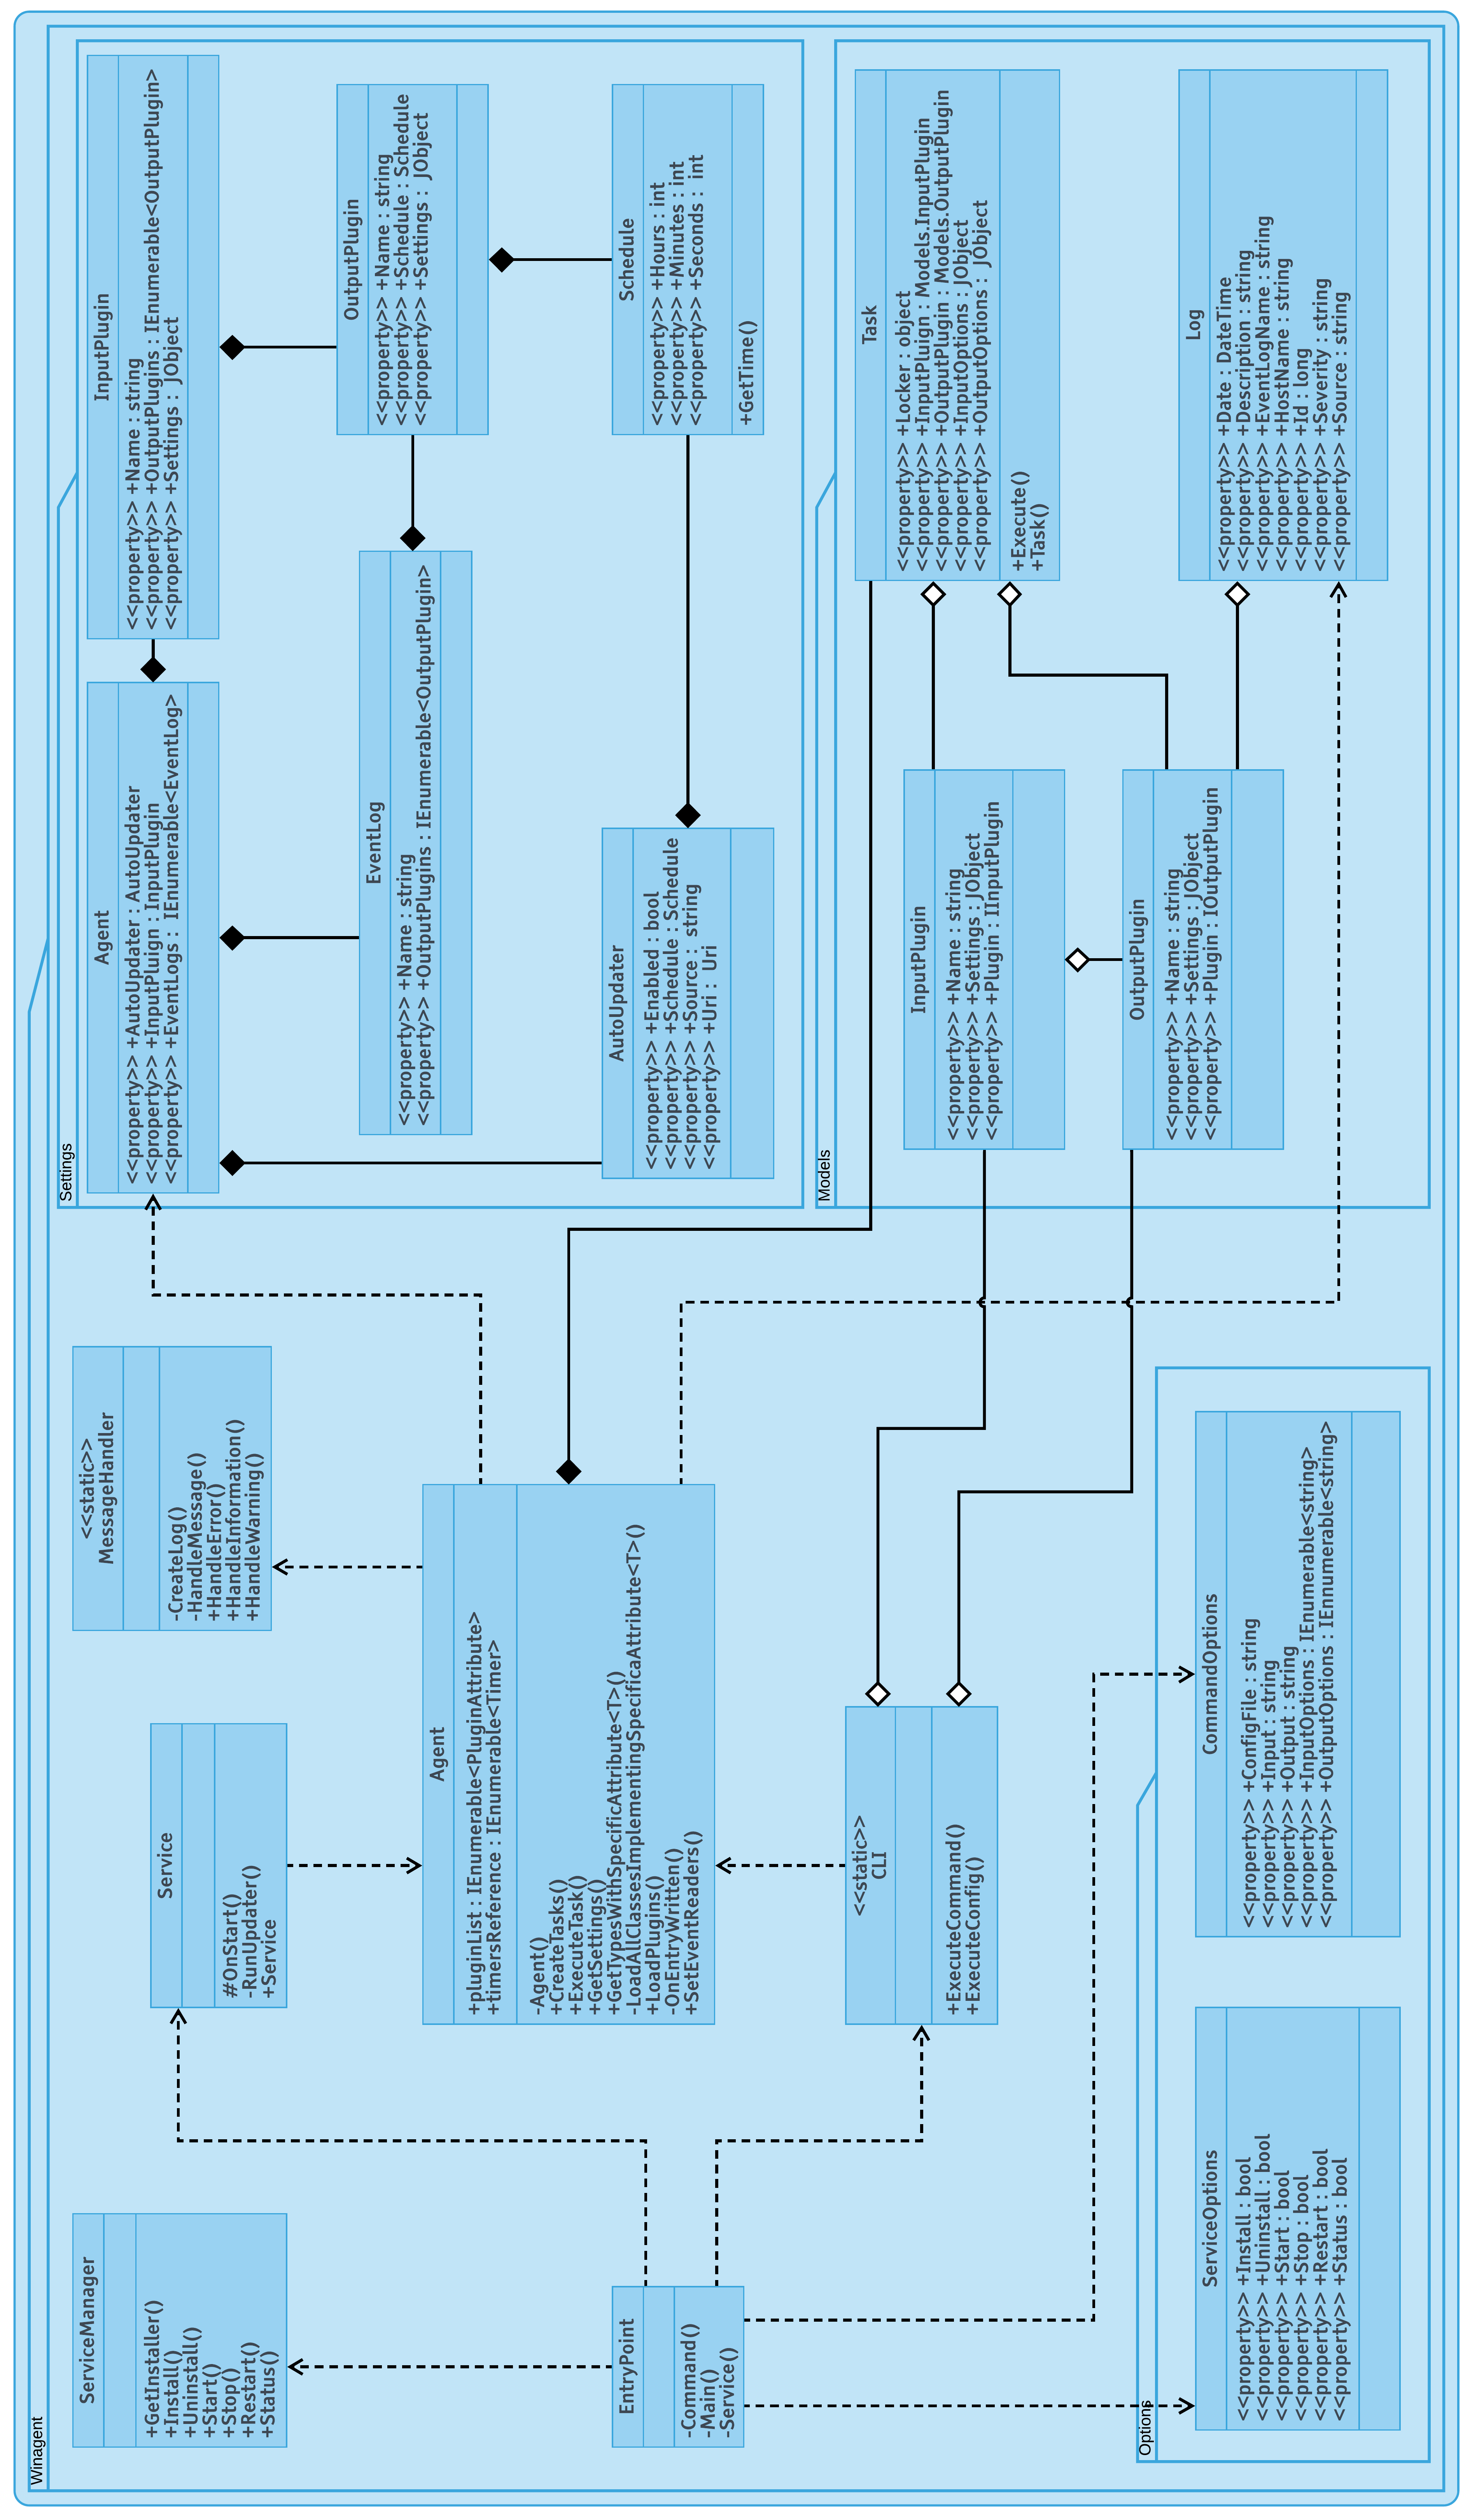
\includegraphics[scale=0.138]{diagrama-de-clases.png}
        \caption{Diagrama de clases}
        \label{fig:class-diagram}
    \end{figure}

    \begin{figure}[H]
    \centering
        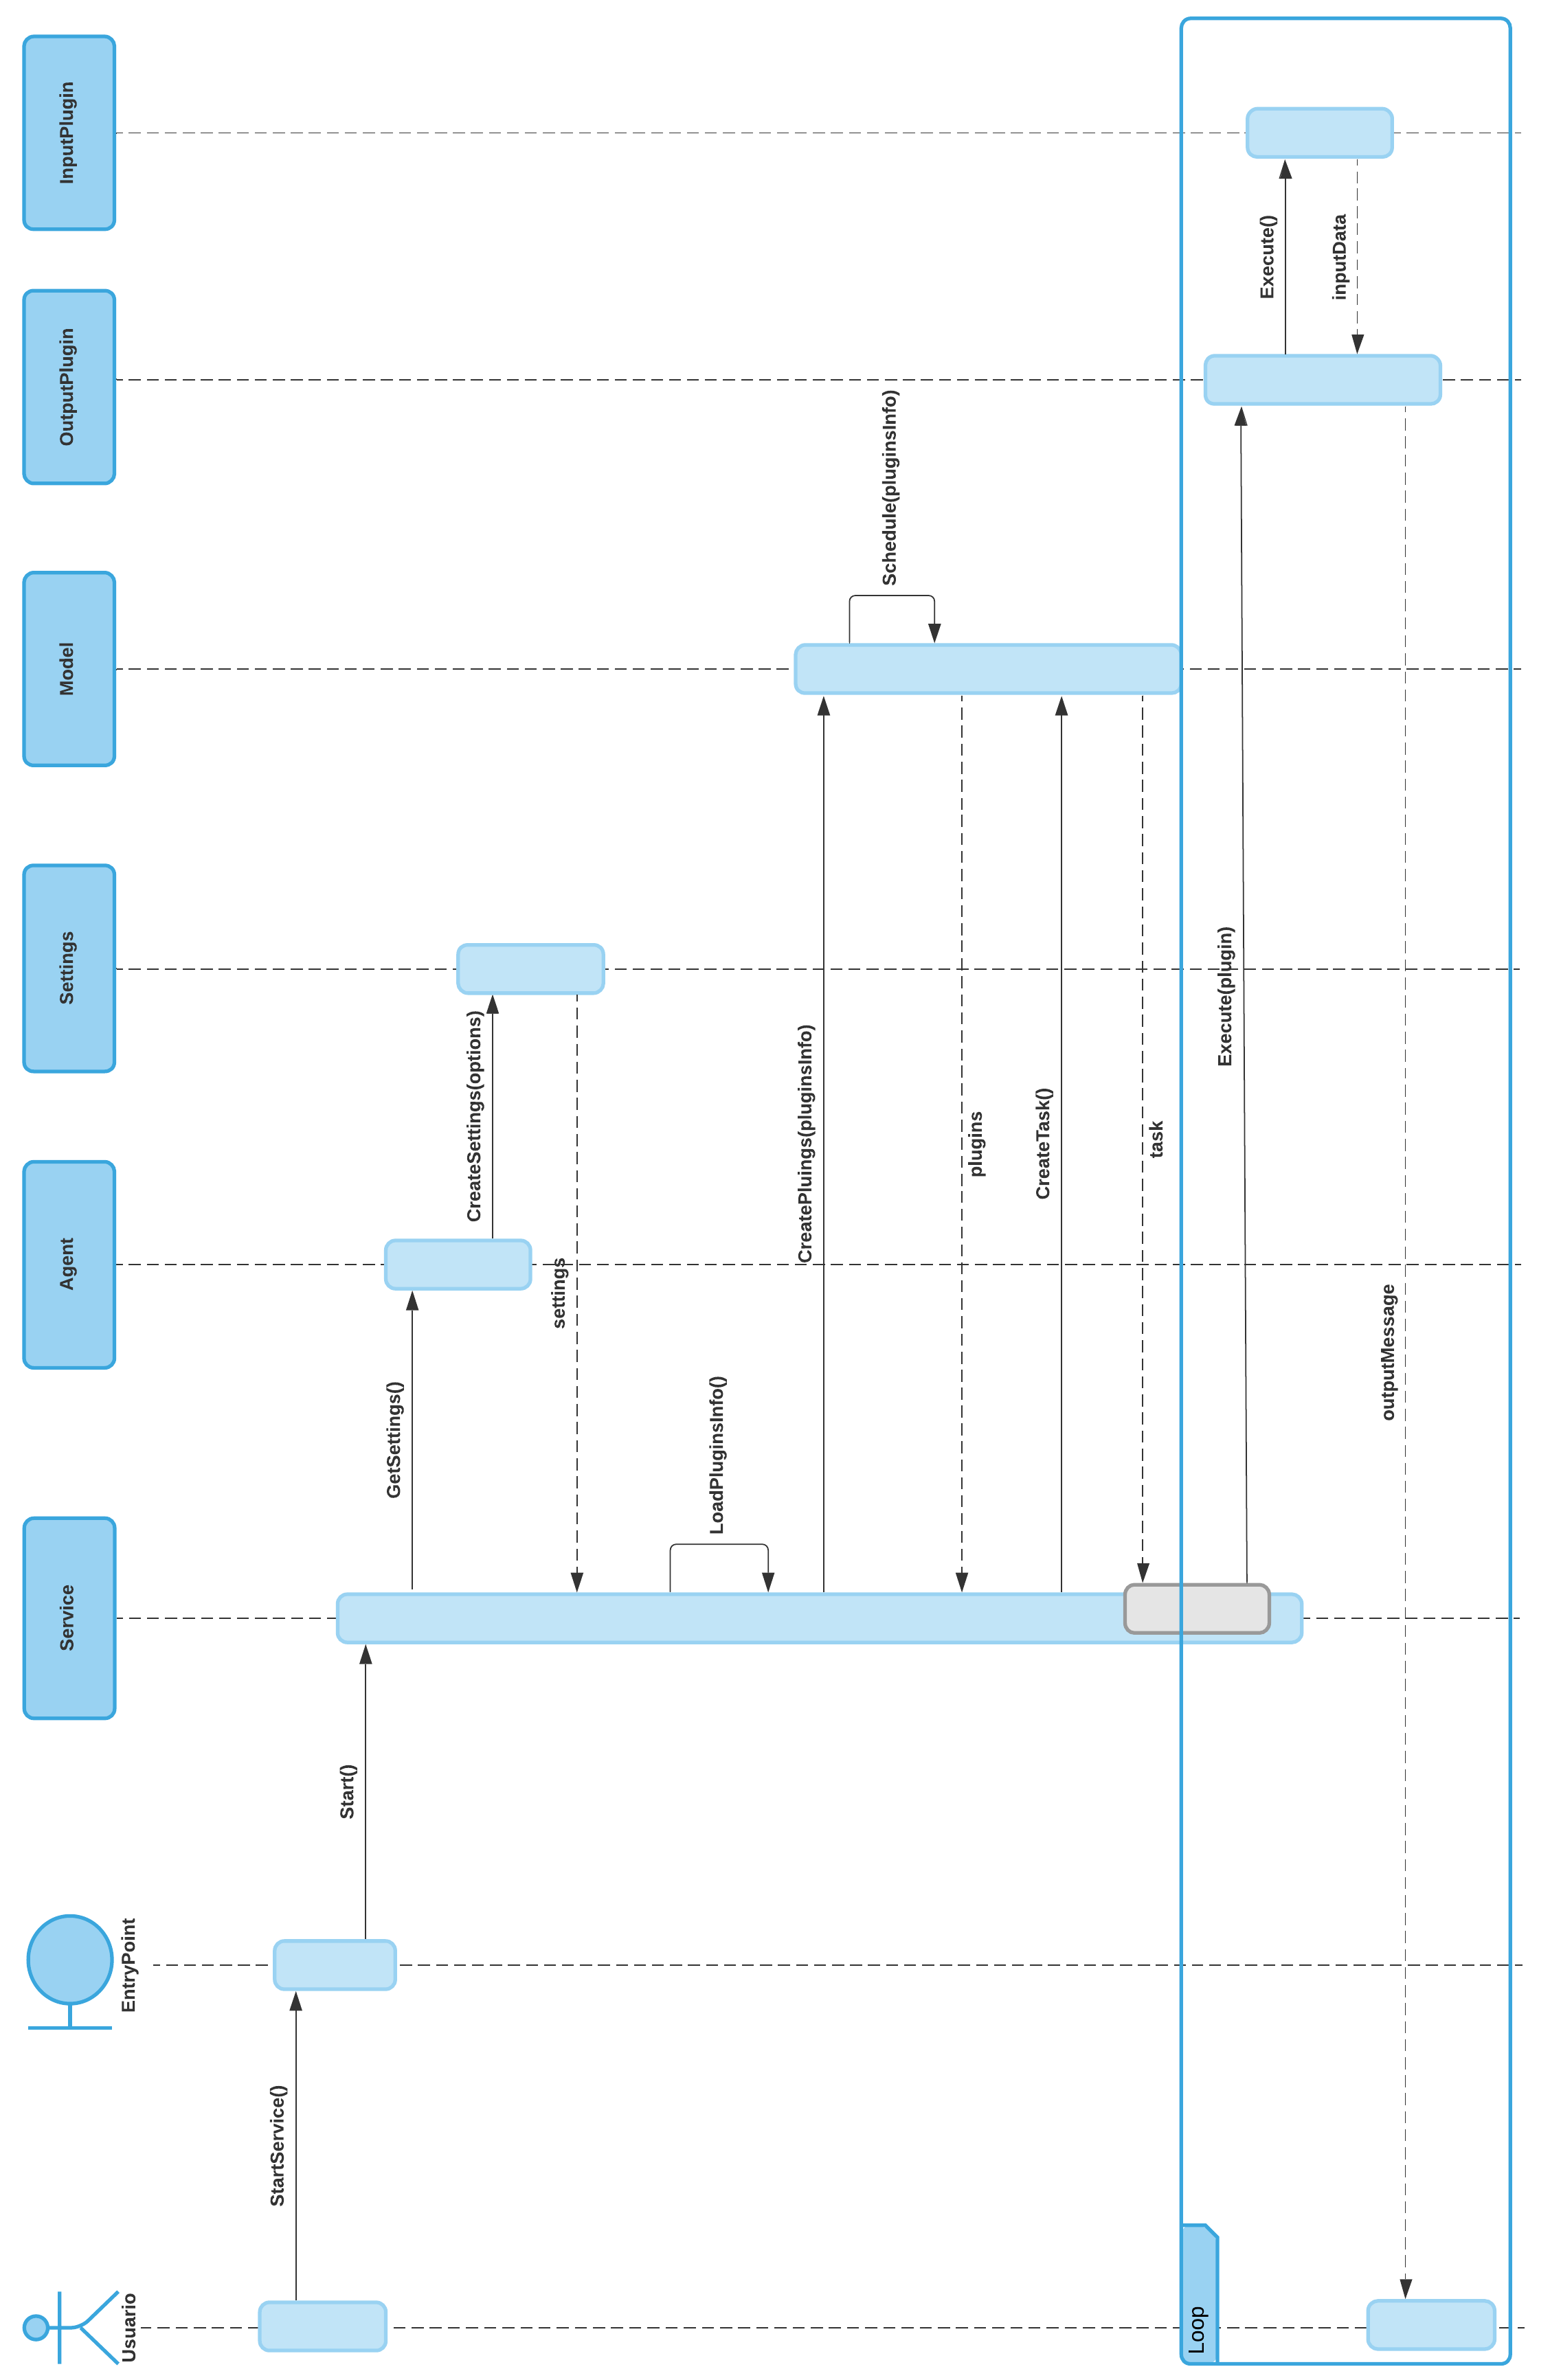
\includegraphics[scale=0.25]{diagrama-secuencia-servicio.png}
        \caption{Diagrama de secuencia - Servicio}
        \label{fig:sequence-diagram-service}
    \end{figure}
    
    \begin{figure}[H]
    \centering
        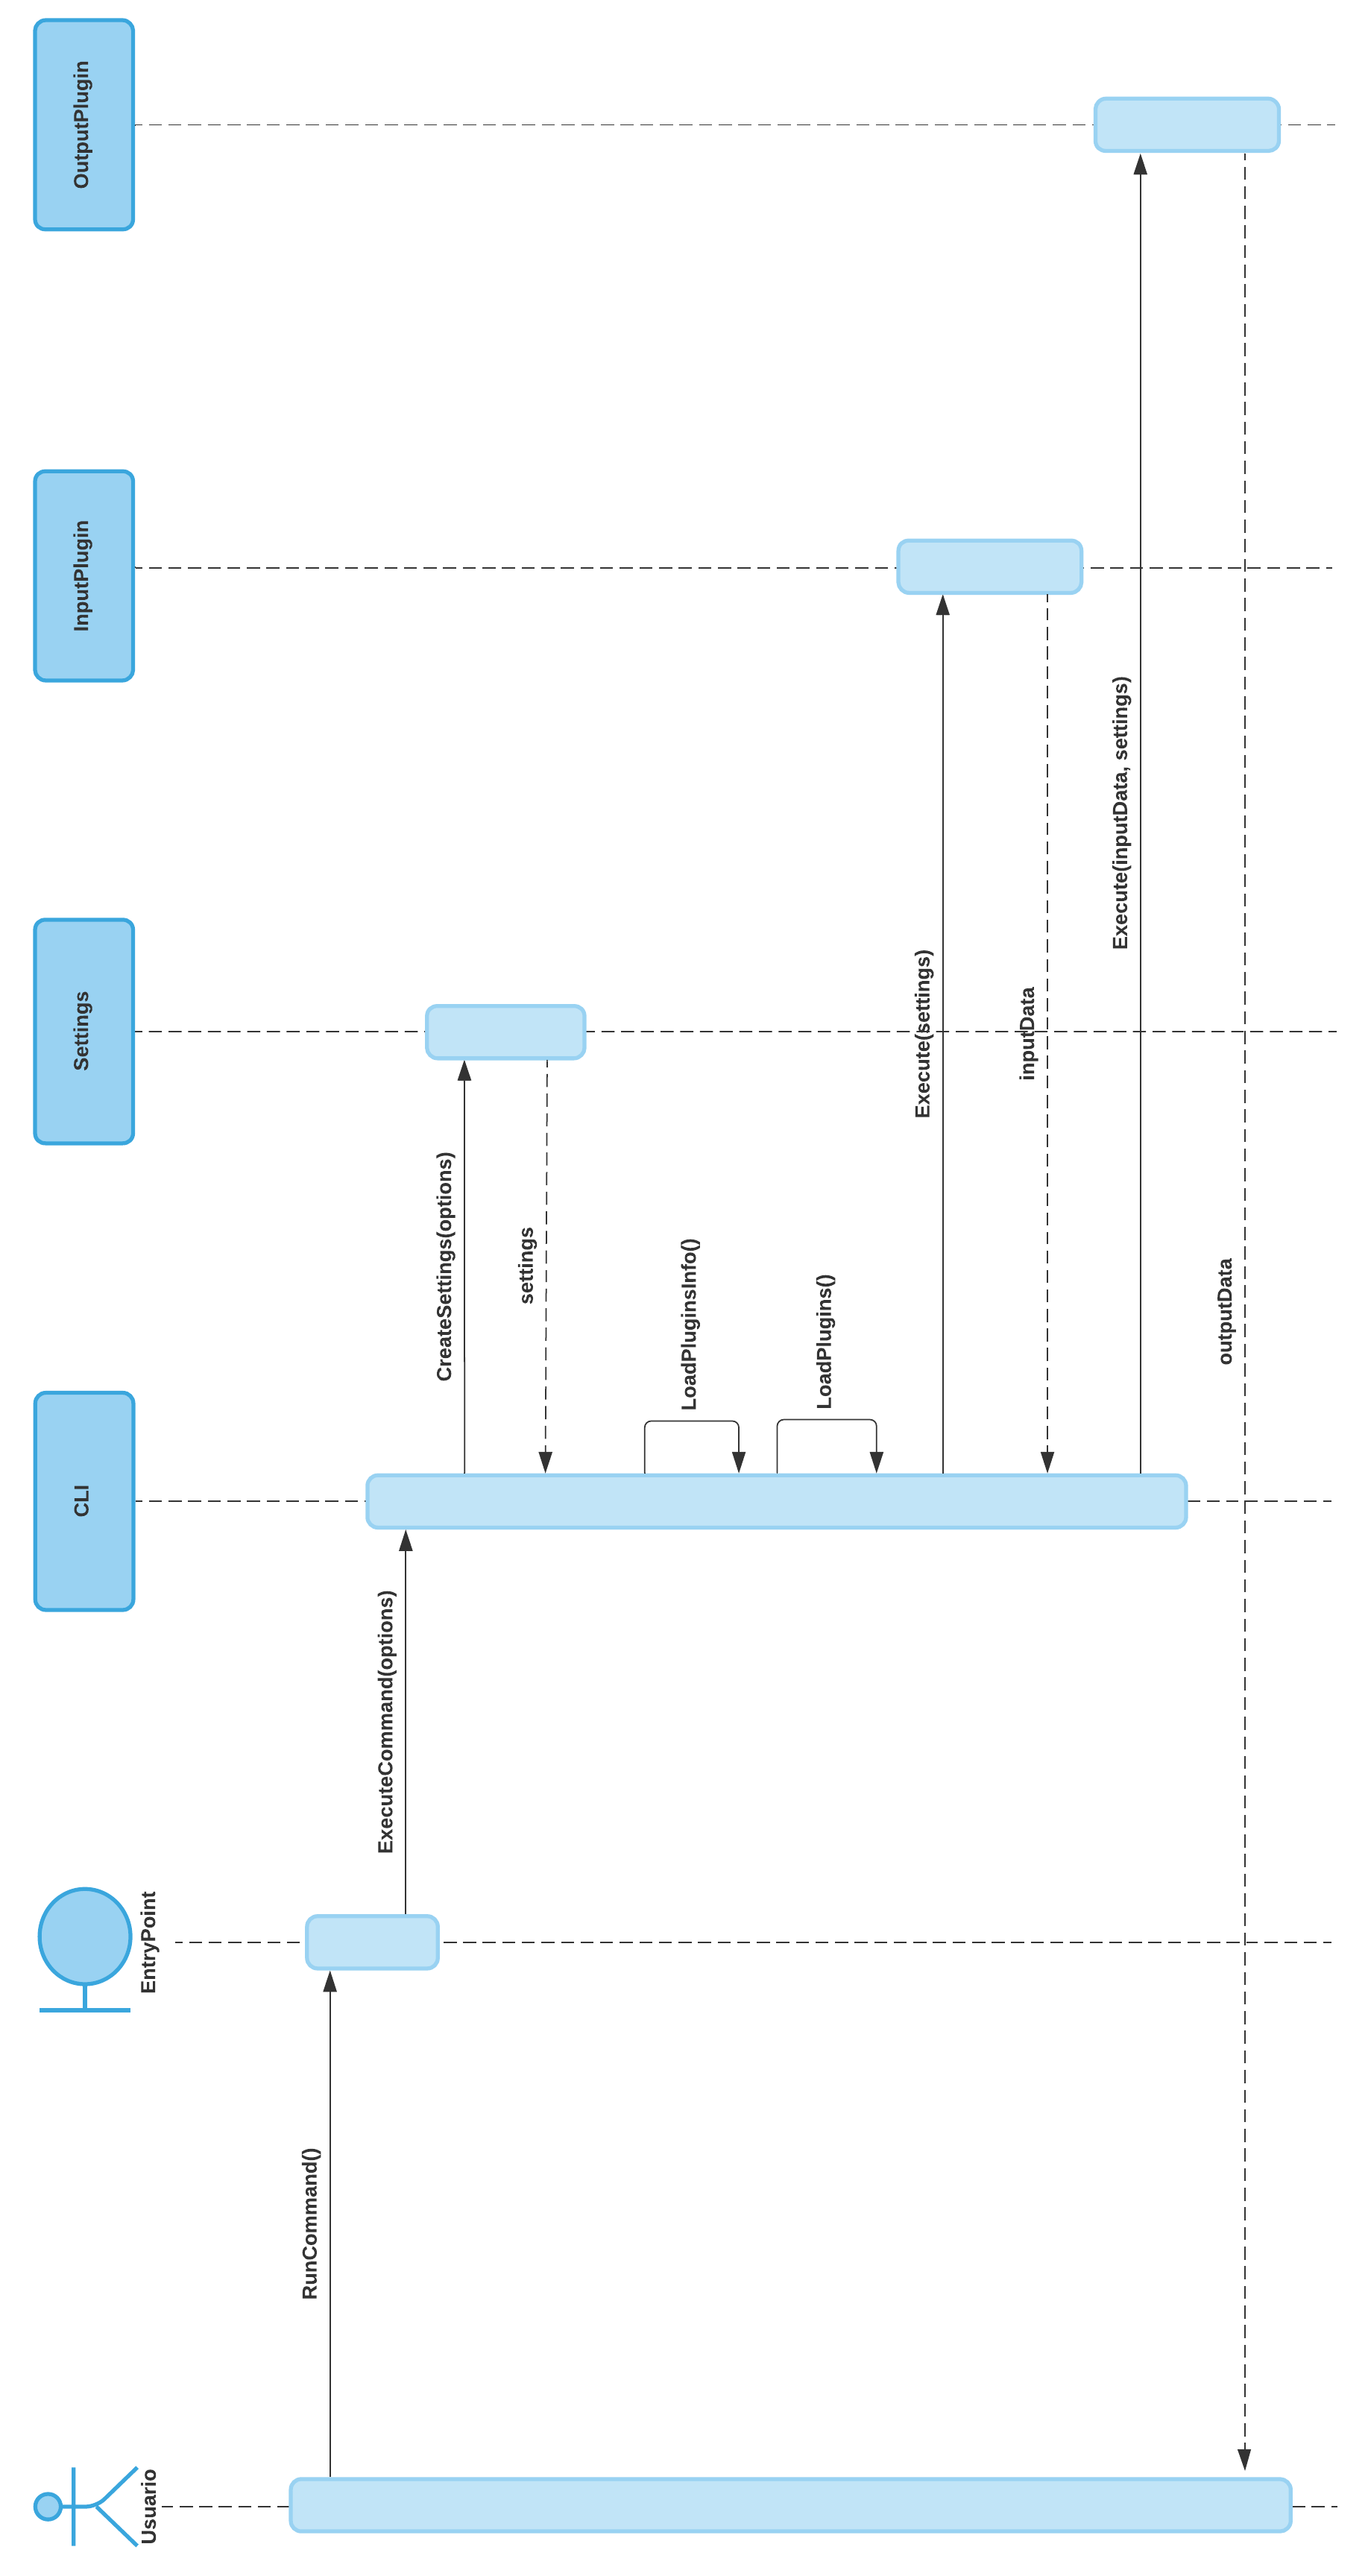
\includegraphics[scale=0.25]{diagrama-secuencia-cli.png}
        \caption{Diagrama de secuencia - \textit{CLI}}
        \label{fig:sequence-diagram-cli}
    \end{figure}
    

% \section{Gestión de datos e información} \label{sec:dat}
% Xestión de datos e información: describiranse os métodos ou técnicas empregadas para xestionar tanto os datos coma o resto de información relevante.
    
\cleardoublepage
\section{Pruebas llevadas a cabo} \label{sec:pru}
% describiranse as probas realizadas aos distintos niveis para
% garantir o correcto funcionamento do software ou do hardware.
    
    Muchos de los paradigmas de programación ágil abarcan el concepto de prueba unitaria. Pruebas programadas en el mismo lenguaje que se escribe la aplicación y que permiten comprobar el funcionamiento de una unidad de código. Sin embargo, dado que desde el inicio del proyecto no estaban claras las fuentes de información que iban a ser utilizadas debido a la gran variedad de librerías y las diferencias entre estas, además de la posibilidad de la adición de cambios en el proyecto que pudiesen cambiar toda su estructura y funcionamiento, se tomó la decisión de no utilizar pruebas automatizadas.
    
    \subsection{Pruebas generales de funcionamiento}
        Para comprobar si el sistema funcionaba correctamente se decidió realizar pruebas manuales, comprobando con cada cambio las funcionalidades previamente desarrolladas. Esto permitiría desarrollar una base del sistema, es decir, alcanzar un punto donde el agente fuese capaz de gestionar correctamente los diferentes \textit{plugins} y hacer uso de estos a través de la \textit{CLI}.
        
    \subsection{Pruebas de funcionamiento como servicio}
        Las pruebas mencionadas anteriormente fueron muy útiles durante el desarrollo de de las funcionalidades principales, sin embargo, probar el servicio supuso una tarea más complicada ya que no era posible mostrar la información en la línea de comandos.
        
        Para comprobar la ejecución del agente al ser utilizado como servició se utilizaron dos métodos, comprobar los sistemas remotos a donde se enviaba la información a ver si llegaba correctamente y los \textit{eventos del sistema} donde se mostraría cualquier información relacionada con el agente en sí.
        
        El desarrollo de un sistema de actualización automática ayudó con las pruebas mencionadas en este apartado, ya que eliminó la necesidad de reiniciar el servicio manualmente y de copiar nuevas versiones de los \textit{plugins} en cada prueba.
    
    \subsection{Pruebas de actualización automática}
        Para comprobar que el sistema de actualización automática funcionara correctamente se utilizaron los \textit{eventos del sistema}, donde se añadirían \textit{logs} para cada acción realizada, como la actualización de algún componente, cualquier tipo de fallo, o un indicador de que el proceso de actualización había terminado.
        
    \subsection{Eventos del sistema}
        Cada \textit{log} creado por el agente o el sistema de actualización automática cuenta con un identificador de evento que permite saber de dónde proviene el mensaje recibido. En el anexo \ref{anx:eventid} se muestra una lista con los identificadores para cada uno de los procesos.
        
    \subsection{Resultados obtenidos}
        En las figuras \ref{fig:rabbitmq-prod-queue} y \ref{fig:rabbitmq-dev-queue} se muestran las colas de dos servidores de \textit{RabbitMQ} (producción y desarrollo), donde se pueden apreciar los resultados de la ejecución como servicio en uno de los servidores \textit{Windows} del \textit{CERN} durante varios días. La configuración utilizada incluye más \textit{plugins} de los inicialmente planteados para este proyecto (\textit{HeartBeat} y \textit{Updates}), los cuales se han mantenido en ejecución por más de una semana.
        
        \begin{figure}[h!]
        \centering
            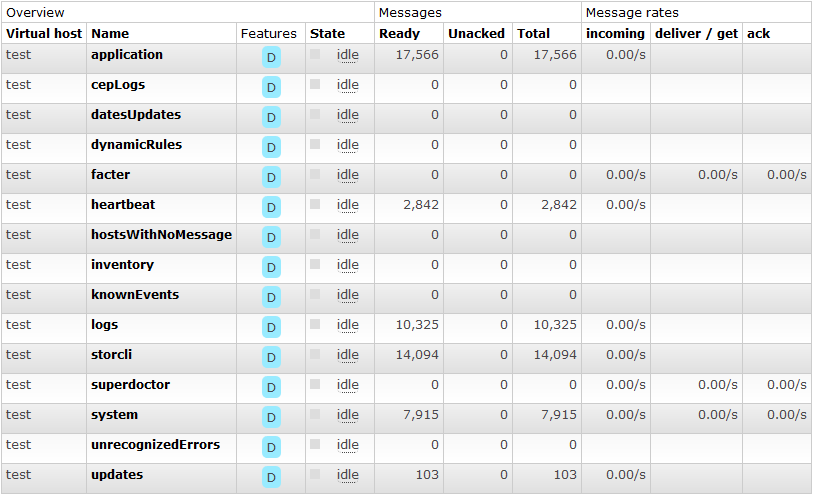
\includegraphics[scale=0.69]{cola-rabbit-mq-prod.png}
            \caption{Colas de RabbitMQ - Producción}
            \label{fig:rabbitmq-prod-queue}
        \end{figure}
    
        \begin{figure}[h!]
        \centering
            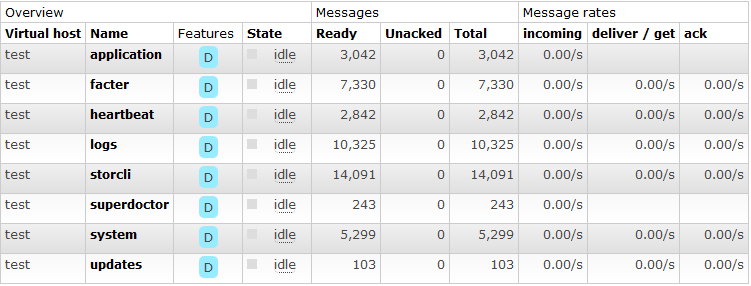
\includegraphics[scale=0.7]{cola-rabbit-mq-dev.png}
            \caption{Colas de RabbitMQ - Desarrollo}
            \label{fig:rabbitmq-dev-queue}
        \end{figure}
        
        Estas imágenes demuestran que hay datos llegando a los servidores \textit{RabbitMQ}, sin embargo, el número de horas de ejecución del agente no coincide con la cantidad de paquetes recibidos para ambos \textit{plugins}. Esto se debe a que la información almacenada en estos servidores incluye mensajes de pruebas anteriores, además de varios reiniciaos del servicio, que hacen que se vuelva a realizar el envío de la información por parte de los \textit{plugins} aunque no haya pasado el tiempo establecido para ello.
        
        En las imágenes \ref{fig:rabbitmq-rate-heartbeat} y \ref{fig:rabbitmq-rate-updates} se pueden apreciar el número de mensajes recibidos en una hora (rango máximo que permiten las gráficas de \textit{RabbitMQ}), esto sí coincide con la configuración aplicada en el servicio, un mensaje de \textit{HeartBeat} cada dos minutos y uno de \textit{Updates} cada una hora.
        
        \begin{figure}[h!]
        \centering
            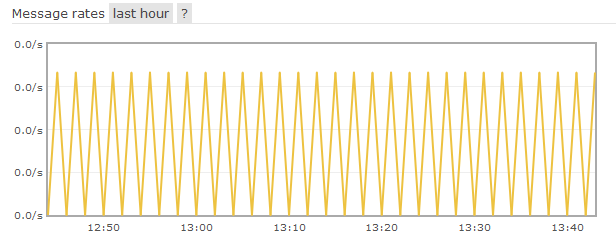
\includegraphics[scale=0.7]{rate-rabbit-mq-heartbeat.png}
            \caption{Mensajes por hora - HeartBeat}
            \label{fig:rabbitmq-rate-heartbeat}
        \end{figure}
        
        \begin{figure}[h!]
        \centering
            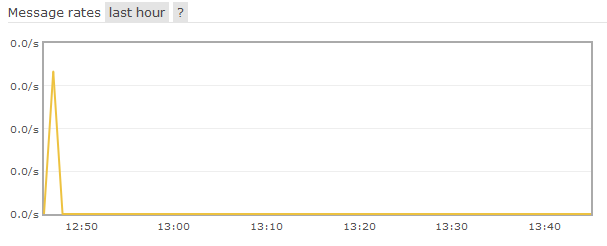
\includegraphics[scale=0.7]{rate-rabbit-mq-updates.png}
            \caption{Mensajes por Hora - Updates}
            \label{fig:rabbitmq-rate-updates}
        \end{figure}
        
\cleardoublepage
\section{Manual de usuario} \label{sec:man}
    En esta sección se detallan los mecanismos de interacción entre el usuario y la aplicación, además de las condiciones necesarias para que esta pueda ser utilizada correctamente. Se debe tener en cuenta que varios de los ejemplos mostrados a continuación son realizados utilizando rutas relativas, es decir, el directorio actual de las demostraciones se corresponde con el de la aplicación. Dependiendo de la consola utilizada es posible que sea necesario indicar la ruta relativa utilizando ``.\textbackslash'' delante del comando a ejecutar o alternativamente se puede utilizar la ruta absoluta, por ejemplo ``C:\textbackslash{}winagent\textbackslash{}winagent.exe''. 

    \subsection{Requisitos mínimos}
        Para poder utilizar \textit{Winagent} no son muchos los requisitos necesarios. El sistema operativo mínimo necesario para su utilización es \textit{Windows 7}, en cuanto a las versiones de escritorio, y \textit{Windows Server 2008} para los servidores.
        
        Se debe tener en cuenta que para instalar el agente como servicio, es necesario tener permisos de \textit{administrador} en el sistema. Además, en caso de utilizar algún \textit{plugin} que tenga dependencias específicas, estas deberán estar presentes en el equipo cuando se lleve a cabo su ejecución.
        
    \subsection{Manual de instalación}
        \subsubsection{Estructura de los archivos}
            Los archivos del sistema deben estar organizados con una estructura concreta, esto permite que todos los \textit{plugins} puedan ser cargados correctamente, al igual que las dependencias y la configuración a ejecutar. A continuación se muestra un ejemplo de dicha estructura y una breve explicación de cada uno de los componentes que se encuentran en ella.
            % TODO: mirar si hay una mejor forma de hacer esto, quizás con el paquete "forest"
            % TODO: Referenciar el diagrama
            \dirtree{%
            .1 winagent.
                .2 plugins.
                    .3 plugin 1.
                    .3 plugin 2.
                    .3 plugin 3.
                .2 tmp.
                    .3 archivo temporal 1.
                    .3 archivo temporal 2.
                .2 dependencia 1.
                .2 dependencia 2.
                .2 plugins.dll.
                .2 winagent.exe.
                .2 winagent-updater.exe.
                .2 config.json.
            }
            
            \begin{itemize}
                \item \textbf{winagent} \\
                    Directorio raíz donde se almacenan los archivos relacionados con el agente en sí, así como las dependencias relacionadas con los \textit{plugins} que lo necesiten.
                    
                \item \textbf{plugins} \\
                    Directorio donde se encuentran todos los \textit{plugins} de entrada y salida que se deseen configurar.
                    
                \item \textbf{tmp} \\
                    Directorio donde se almacenan de forma temporal los archivos que son descargados por el actualizador automático. Esto incluye los archivos relacionados con el agente, \textit{plugins} y \textit{hashes} para comprobar la integridad de los archivos descargados.
                    
                \item \textbf{plugin.dll} \\
                    Interfaz de la que dependen todos los \textit{plugins} de la aplicación, es utilizada por el agente durante el proceso de carga para detectar todos componentes que la implementan.
                
                \item \textbf{winagent.exe} \\
                    Ejecutable del agente, utilizado desde la \textit{CLI} y por el servicio una vez instalado.
                
                \item \textbf{winagent-updater.exe} \\
                    Ejecutable del sistema de actualización automática, es lanzado directamente por el agente en intervalos programados.
                
                \item \textbf{config.json} \\
                    Archivo de configuración donde se almacenan todos los ajustes por los que se rigen tanto el agente como el proceso de actualización automática durante sus ejecuciones.
                
            \end{itemize}
            
        \subsubsection{Instalación del servicio}
            Con la finalidad de que \textit{Winagent} pueda funcionar como un servicio, primeramente deberá ser instalado como tal. Este proceso requiere que el usuario que lo realiza cuente con permisos de administrador. Para llevar a cabo la instalación puede ser utilizada cualquiera de las herramientas disponibles en el sistema operativo o el verbo \textit{service} junto con la opción \textit{-{}-install} de la propia aplicación.
            
            A continuación se muestran varias formas de instalar \textit{Winagent} utilizando diferentes métodos.
            
            \begin{lstlisting}[style=batch, caption=Instalación el servicio utilizando el propio agente]
                > winagent.exe service --install
            \end{lstlisting}
            
            \begin{lstlisting}[style=batch, caption=Instalación el servicio mediante la utilidad \textit{InstallUtil}]
                > InstallUtil winagent.exe
            \end{lstlisting}
            
            \begin{lstlisting}[style=batch, caption=Instalación el servicio utilizando \textit{PowerShell}]
                > New-Service -Name "Winagent" -BinaryPathName "C:\winagent\winagent.exe"
            \end{lstlisting}
            
     \subsection{Manual de utilización}
        \subsubsection{CLI}
            A través de la interfaz de línea de comandos que brinda el agente se puede hacer uso de todas sus funcionalidades utilizando el verbo \textbf{\textit{run}}. Para ello existen dos métodos, indicando manualmente las opciones en el comando ejecutado o especificando un archivo de configuración donde se encuentren definidos todos los ajustes a emplear.
            
            Al utilizar el verbo \textbf{\textit{run}}, por defecto, se utiliza el \textit{plugin de entrada} ``updates'' y el \textit{plugin de salida} ``output'', que es el que permite que los resultados sean mostrados en la consola.
            
            \begin{lstlisting}[style=batch, caption=Ejecución por defecto]
                > winagent.exe run
            \end{lstlisting}
            
            Las opciones \textit{-{}-input/-i} y \textit{-{}-output/-o} sirven para especificar manualmente los \textit{plugins} que son ejecutados. El resultado obtenido al utilizar el comando anterior sería exactamente igual al del siguiente comando:
            
            \begin{lstlisting}[style=batch, caption=Ejecución de forma manual]
                > winagent.exe run -i updates -o console
            \end{lstlisting}
            
            Además, también se pueden especificar las opciones necesarias para cada uno de los \textit{plugins} que se desea ejecutar. En el siguiente ejemplo se muestra cómo imprimir en pantalla los datos con un formato de tabla, indicando un valor de ``outputType'' al \textit{plugin} de salida. Para esto se deben utilizar las opciones ``input-options'' y ``output-options'', pudiendo especificar varias separándolas mediante comas(,).
            
            \begin{lstlisting}[style=batch, caption=Ejecución de forma manual]
                > winagent.exe run -o console --output-option outputType:table
            \end{lstlisting}

            Para utilizar un fichero de configuración, simplemente se debe indicar la ruta a este. Una vez iniciado, el agente carga los \textit{plugins} definidos, los cuales son ejecutados en los intervalos especificados. Para terminar la ejecución basta con presionar cualquier tecla.
            
            \begin{lstlisting}[style=batch, caption=Ejecución utilizando un fichero de configuración]
                > winagent.exe run C:\winagent\config.json
            \end{lstlisting}
        
        \subsubsection{Servicio}
        
            Cuando el agente es utilizado como servicio, se ejecuta en segundo plano y utiliza los ajustes especificados en un fichero de configuración nombrado \textit{config.json} que se encuentre su misma carpeta.
            
            Además, \textit{Winagent} cuenta con una herramienta que permite administrar el servicio a través de una consola de comandos, utilizando el verbo \textbf{\textit{service}}. A continuación se describen los comandos disponibles y su funcionalidad.
            
            \begin{lstlisting}[style=batch, caption=Instalar el servicio]
                > winagent.exe service --install
            \end{lstlisting}
            
            \begin{lstlisting}[style=batch, caption=Desinstalar el servicio]
                > winagent.exe service --uninstall
            \end{lstlisting}
            
            \begin{lstlisting}[style=batch, caption=Iniciar el service]
                > winagent.exe service --start
            \end{lstlisting}
            
            \begin{lstlisting}[style=batch, caption=Detener el servicio]
                > winagent.exe service --stop
            \end{lstlisting}
            
            \begin{lstlisting}[style=batch, caption=Reiniciar el servicio]
                > winagent.exe service --restart
            \end{lstlisting}
            
            \begin{lstlisting}[style=batch, caption=Comprobar el estado del servicio]
                > winagent.exe service --status
            \end{lstlisting}
            
        \subsubsection{Archivo de configuración}
            En el archivo de configuración se deben establecer todos los ajustes con los que se desea ejecutar el agente. Este debe tener una estructura específica que incluye información utilizada por el actualizador, los lectores de eventos del sistema, los \textit{plugins} de entrada y salida, y las opciones con las que se ejecutarán estos. A continuación se muestra la estructura básica que debe tener este fichero, mientras que en el anexo \ref{anx:settings} se puede apreciar un ejemplo real con el contenido de un archivo que ya ha sido puesto en producción.
            
            % TODO: crear estilo para archivo de configuracion
            \begin{lstlisting}[style=csharp, caption=Fichero de configuración]
                {
                  "autoUpdates": {
                    "enabled": true,
                    "source": "gitlab / github",
                    "uri": "ReleaseURL",
                    "schedule": {
                      "seconds": 0,
                      "minutes": 0,
                      "hours": 0
                    }
                  },
                  "eventLogs": [
                    {
                      "name": "Application",
                      "outputPlugins": [
                        {
                            "name": "OutputPluginName",
                            "settings": {
                              "SettingName": "SettingValue"
                            },
                            "schedule": {
                              "seconds": 0,
                              "minutes": 0,
                              "hours": 0
                            }
                        }
                      ]
                    }
                  ],
                  "inputPlugins": [
                    {
                      "name": "InputPluginName",
                      "settings": {
                          "SettingName": "SettingValue"
                      },
                      "outputPlugins": [
                        {
                          "name": "OutputPluginName",
                          "settings": {
                            "SettingName": "SettingValue"
                          },
                          "schedule": {
                            "seconds": 0,
                            "minutes": 0,
                            "hours": 0
                          }
                        }
                      ]
                    }
                  ]
                }
            \end{lstlisting}
            
            
    \red{PONER UN MANUAL DE CONFIGURACIÓN DE LOS PLUGINS DESARROLLADOS}
        
    \subsection{Manual de desarrollo}
        Una de las características principales de \textit{Winagent} es que permite el desarrollo de nuevos \textit{plugins} que puedan ser combinados con los ya existentes sin modificar la aplicación, permitiendo obtener diferente información y utilizarla en nuevos sistemas. A continuación se muestran dos ejemplos y se especifican los pasos necesarios para la creación de librerías que puedan ser utilizadas como \textit{plugins}.
        
        \begin{enumerate}
            \item Compilar la librería base de los plugins. Puede ser encontrada tanto en GitHub como en GitLab.
            
            https://gitlab.cern.ch/winagent/plugin
            
            https://github.com/cern-winagent/plugin
            
            \item Utilizando \textit{Visual Studio}, crear una \textit{Biblioteca de Clases (.NET Framework)}
            
            \item Añadir la \textit{dll} compilada en el paso 1 como referencia al nuevo proyecto
            
            \item Crear una clase llamada \textit{I[nombre del plugin]} u \textit{O[nombre del plugin]} que implemente la interfaz \textit{IInputPlugin} o \textit{IOutputplugin} respectivamente.
            
            \item Nombrar el \textit{plugin} utilizando el atributo \textit{PluginName}.
            
            \item Implementar el método \textit{Execute}, donde se especifican las funciones que realizará el \textit{plugin}.
        \end{enumerate}
    
        \begin{lstlisting}[style=csharp, caption=Plugin de entrada]
            namespace plugin
            {
                /// <summary>
                ///     This class implements the custom attribute required
                ///     by the agent to be recognized as a plugin.
                /// </summary>
                [PluginAttribute(PluginName = "Updates")]
                public class IUpdates : IInputPlugin
                {
                    /// <summary>
                    ///     Runs the main functionality of the plugin.
                    ///     Normally used to get system information.
                    /// </summary>
                    /// <param name="settings">
                    ///     Settings to be used inside the plugin.
                    /// </param>
                    /// <returns>
                    ///     A string formated as JSON.
                    /// </returns>
                    public string Execute(JObject settings)
                    {
                        ...
            
                        return jsonstring;
                    }
                }
            }
        \end{lstlisting}
        
        \begin{lstlisting}[style=csharp, caption=Plugin de salida]
            namespace plugin
            {
                [PluginAttribute(PluginName = "Console")]
                public class OConsole : IOutputPlugin
                {
                
                    /// <summary>
                    ///     Runs the main functionality of the plugin.
                    ///     Normally used to show or send to another
                    ///     system the information received.
                    /// </summary>
                    /// <param name="settings">
                    ///     Settings to be used inside the plugin.
                    /// </param>
                    public void Execute(string data, JObject settings)
                    {
                        ...
                    }
                }
            }
        \end{lstlisting}


% conclusion %
\chapter{Conclusiones}
\label{sec:conc}
\section{Principales aportaciones}
% deberanse destacar entre 3 e 5 aportacións importantes do
% traballo realizado, tendo en conta os obxectivos fixados.
    Teniendo en cuenta los objetivos planteados, este proyecto contiene un conjunto de aportaciones entre las que se pueden destacar:
    
    \begin{itemize}
        \item Creación de un mecanismo de obtención de datos capaz de transmitir información de forma periódica a los servicios necesarios.
        
        \item Se ha creado un sistema modular al cual le pueden ser ampliadas sus funcionalidades mediante la adición de librerías, sin necesidad de modificar el código fuente de la aplicación.
        
        \item Se ha incorporado un mecanismo de actualización automática, que permite mantener la aplicación actualizada sin necesidad de acceder manualmente a los servidores donde esté instalada para modificarla.
        
        \item Se ha proporcionado un mecanismo de monitorización, que permite leer en tiempo real los \textit{EventLogs} y transmitirlos a diferentes sistemas de forma configurable.
        
        \item Se brindan nuevas opciones para la depuración de fallos, mediante una interfaz de línea de comandos capaz de obtener toda la información que pueda proporcionar el agente sin necesidad de estar instalado. Estos datos pueden ser mostrados de forma local o enviados manualmente a otros sistemas remotos.
    \end{itemize}







% incluiranse todas as conclusións de tipo técnico e persoal.

    Mantener el control de las actualizaciones, reportes de discos duros y otros reportes de sistema en más de mil servidores, es un problema al que se han enfrentado durante años los administradores del \textit{CERN}. Este \textit{Trabajo de Fin de Máster} ha intentado facilitar esta tarea, de forma tal que se abarcasen todos los casos de uso de interés, y proveyendo un mecanismo integrable para cubrir otros que puedan surgir en el futuro.
    
    Tras un largo proceso de desarrollo, este proyecto llega a su fin, y, pese a haber supuesto más tiempo del planificado debido a los diferentes cambios introducidos, se considera que todos los objetivos propuestos han sido alcanzados. Además, es interesante mencionar que estos cambios han ayudado a obtener un sistema mucho más sólido que ya se ha puesto en producción satisfactoriamente.
    
    En el plano personal, me siento satisfecho de haber realizado este proyecto que representa un gran paso de avance dentro del CERN. Llevar a cabo su desarrollo me ha permitido ampliar mis conocimientos ya que he utilizando \textit{.NET} y \textit{CSharp}, un lenguaje de programación en el que no tenía experiencia  hasta comenzar con este proyecto. Además, aunque haya sido un proyecto de desarrollo individual, me ha dado la oportunidad de colaborar con fantásticos compañeros lo cual me ha ayudado a entender los problemas y necesidades de los sistemas que ahora dependen de esta aplicación y así poder encontrar la solución mas adecuada.


\section{Trabajo futuro}
% presentaranse posible ampliacións e traballos relacionados por facer.
        
    Aunque el planteado en este proyecto ha sido alcanzado y es sistema al cual le red{pueden ser añadidos} una innumerable cantidad de funcionalidades a través de los plugins , no \red{caben} dudas de que aún puede ser mejorado, ya sea añadiendo nuevas funcionalidades en el propio agente, o mejorando las tareas que realiza para \red{proveer} una mejor eficiencia o brindar más control sobre el producto.
    
    A continuación se listan posibles mejoras que pueden ser añadidas al proyecto en un futuro.
            
    \subsection{Generador de configuraciones}
        El hecho de que el sistema sea \red{muy} flexible hace que el usuario deba especificar en un archivo de configuración todos los ajustes necesarios para su ejecución. Debido a esto, la complejidad de este archivo puede llegar a ser muy alta, por lo que el usuario es propenso a cometer algún error durante su creación, lo que llevaría a un error durante la ejecución de la aplicación.
        
        Para solventar este problema, sería muy útil implementar un sistema que permitiese crear los archivos de configuración de forma semi-automática. De esta forma, para obtener el contenido \textit{.JSON} con una configuración libre de errores, el usuario solo debería seleccionar los plugins que desee y rellenar los campos necesarios.
        
    \subsection{Soporte flexible para \textit{APIs} en el sistema de actualización automática}
        El sistema de actualización automática implementado brinda soporte para las \textit{APIs} de \textit{GitHub} y \textit{GitLab}. Desde estas puede obtener la información necesaria acerca de los ficheros a actualizar, sin embargo, está limitado a la estructura de estas, por los que son las únicas fuentes que pueden ser utilizadas.
        
        Se podría crear un mecanismo que tomara la estructura de la \textit{API} desde el fichero de configuración, de forma que el usuario pueda establecerla manualmente. Esto permitiría el uso de \textit{APIs} personalizadas, pudiendo acceder a cualquiera de sus elementos.

    \subsection{Paquete \textit{MSI}}
        El sistema desarrollado es puede ser instalado y ejecutado como un servicio, además de que tiene la capacidad de ser actualizado de forma automática en períodos configurables. No obstante, el despliegue de la aplicación se realiza mediante \textit{scripts} cuyo objetivo es copiar todos los archivos y realizar las instalaciones pertinentes en cada uno de los servidores.
        
        Una solución a esta limitación sería la creación de un \textit{Instalador de Windows (.msi)} \cite{msi}, un paquete desplegable que contenga los archivos del sistema junto con todas sus dependencias, y realice su instalación de forma automática. Esto representa una gran \red{ventaja}, ya que es un tipo de instalador que puede ser desplegado fácilmente en varios sistemas mediante el uso de \textit{herramientas de gestión de configuración} \cite{configmanag} como \textit{Puppet}\cite{puppet} o directamente desde \textit{Active Directory}, herramientas que son actualmente utilizadas en el \textit{CERN}.

    \subsection{Detectar cambios en la configuración}
        Dado que la configuración del agente es leída justo después de haber iniciado el sistema, cualquier cambio realizado en esta es ignorado hasta que el servicio sea reiniciado. Esto implica que si se desea realizar un cambio, se deberá reiniciar el servicio de forma manual o esperar a que ocurra una actualización de alguno de los componentes.
        
        Para solucionar esto se deberá crear un mecanismo que \red{se mantenga pendiente} del archivo de configuración con el que fue ejecutado el sistema, y una vez detecte algún cambio en este, reinicie el servicio de forma automática.



% conclusion %
\chapter{Anexos}
\appendix % TODO: Revisar anexos y fotos con títulos
\section{RAID 1}\label{anx:raid1}
    \begin{figure}[h!]
    \centering
        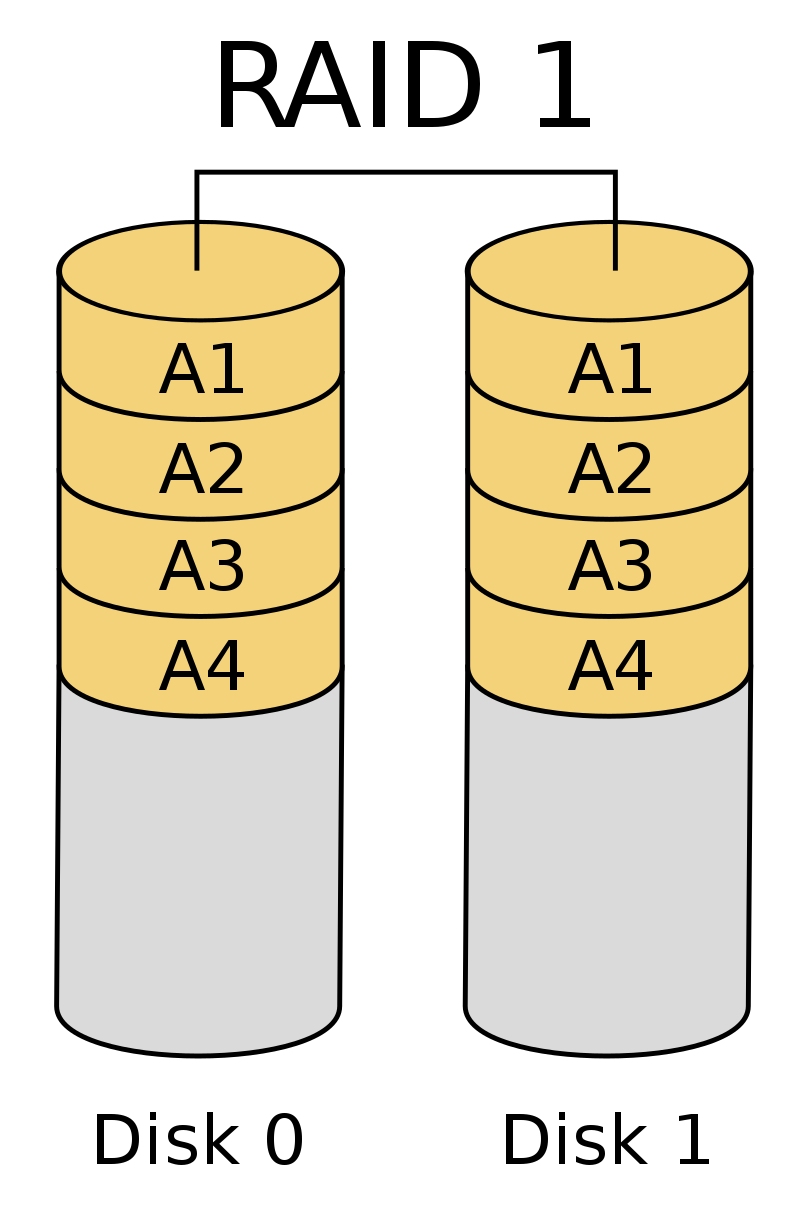
\includegraphics[scale=0.2]{raid1.png}
        \caption{Estructura RAID1}
        \label{fig:raid1}
    \end{figure}
    
\section{Filtro de errores}\label{anx:hw-info}
    \begin{figure}[h!]
    \centering
        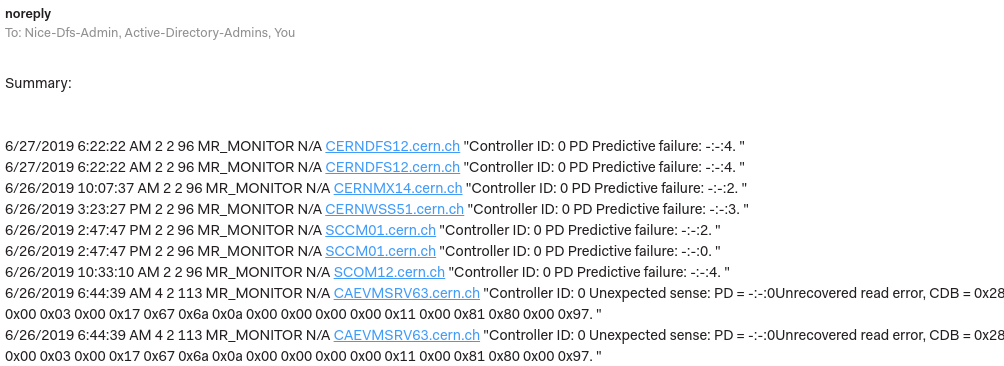
\includegraphics[scale=0.55]{filtro-de-errores.png}
        \caption{Filtro de errores de \textit{hardware}}
        \label{fig:error-filter}
    \end{figure}
    
\section{Listado de \textit{EventIDs} utilizados}\label{anx:eventid}
    \textbf{Winagent}
        \begin{enumerate}
            \setcounter{enumi}{-1}
            \item Error durante la administración del servicio
            \item Ha ocurrido un error general
            \item Error ejecutando el actualizador
            \item Se ha actualizado el sistema de actualización automática
            \item No hay \textit{plugins} que ejecutar
            \item Error al ejecutar un \textit{plugin}
            \item Archivo de configuración no encontrado.
            \item Error en el archivo de configuración
            \item Error obteniendo datos del archivo de configuración
            \item Archivos inválidos en la carpeta ``plugins''
            \item Error mientras se lanzaba un evento
            \item No se pudo encontrar el ejecutable del actualizador
            \item Ejecución de los \textit{plugins} superpuesta
        \end{enumerate}{}
        
        \textbf{Actualizador automático}
        \begin{enumerate}
            \setcounter{enumi}{-1}
            \item Error general del sistema
            \item Petición HTTP fallida
            \item Servicio no iniciado
            \item No se pudo guardar un archivo
            \item No se pudo encontrar el directorio ``tmp''
            \item No se pudo encontrar la ruta al archivo de configuración
            \item Error en el archivo de configuración
            \item Error obteniendo datos del archivo de configuración
            \item Componente actualizada
        \end{enumerate}{}
        
    
    \section{Ejemplo de configuración real}\label{anx:settings}
        \begin{lstlisting}[style=csharp, caption=Fichero de configuración]
            {
              "autoUpdates": {
                "enabled": true,
                "source": "gitlab",
                "uri": "https://gitlab.cern.ch/api/v4/projects/winagent%2F{plugin}/releases/production",
                "schedule": {
                  "seconds": 0,
                  "minutes": 5,
                  "hours": 1
                }
              },
              "eventLogs": [
                {
                  "name": "Application",
                  "outputPlugins": [
                    {
                      "name": "RabbitMQ",
                      "settings": {
                        "servers": [
                          {
                            "hostName": "restricted.cern.ch",
                            "userName": "restricted",
                            "password": "restricted",
                            "queueName": "logs",
                            "virtualHost": "test"
                          },
                          {
                            "hostName": "restricted.cern.ch",
                            "userName": "restricted",
                            "password": "restricted",
                            "queueName": "logs",
                            "virtualHost": "test"
                          }
                        ]
                      }
                    }
                  ]
                },
                {
                  "name": "System",
                  "outputPlugins": [
                    {
                      "name": "RabbitMQ",
                      "settings": {
                        "servers": [
                          {
                            "hostName": "restricted.cern.ch",
                            "userName": "restricted",
                            "password": "restricted",
                            "queueName": "logs",
                            "virtualHost": "test"
                          },
                          {
                            "hostName": "restricted.cern.ch",
                            "userName": "restricted",
                            "password": "restricted",
                            "queueName": "logs",
                            "virtualHost": "test"
                          }
                        ]
                      }
                    }
                  ]
                }
              ],
              "inputPlugins": [
                {
                  "name": "Storcli",
                  "settings": {
                  },
                  "outputPlugins": [
                    {
                      "name": "RabbitMQ",
                      "settings": {
                        "servers": [
                          {
                            "hostName": "restricted.cern.ch",
                            "userName": "restricted",
                            "password": "restricted",
                            "queueName": "Storcli",
                            "virtualHost": "test"
                          },
                          {
                            "hostName": "chopin-amqp-d.cern.ch",
                            "userName": "restricted",
                            "password": "restricted",
                            "queueName": "Storcli",
                            "virtualHost": "test"
                          }
                        ]
                      },
                      "schedule": {
                        "seconds": 0,
                        "minutes": 2,
                        "hours": 0
                      }
                    }
                  ]
                },
                {
                  "name": "Facter",
                  "settings": {
                  },
                  "outputPlugins": [
                    {
                      "name": "RabbitMQ",
                      "settings": {
                        "servers": [
                          {
                            "hostName": "restricted.cern.ch",
                            "userName": "restricted",
                            "password": "restricted",
                            "queueName": "Facter",
                            "virtualHost": "test"
                          },
                          {
                            "hostName": "restricted.cern.ch",
                            "userName": "restricted",
                            "password": "restricted",
                            "queueName": "Facter",
                            "virtualHost": "test"
                          }
                        ]
                      },
                      "schedule": {
                        "seconds": 0,
                        "minutes": 2,
                        "hours": 0
                      }
                    }
                  ]
                },
                {
                  "name": "Updates",
                  "settings": {
                  },
                  "outputPlugins": [
                    {
                      "name": "RabbitMQ",
                      "settings": {
                        "servers": [
                          {
                            "hostName": "restricted.cern.ch",
                            "userName": "restricted",
                            "password": "restricted",
                            "queueName": "Updates",
                            "virtualHost": "test"
                          },
                          {
                            "hostName": "restricted.cern.ch",
                            "userName": "restricted",
                            "password": "restricted",
                            "queueName": "Updates",
                            "virtualHost": "test"
                          }
                        ]
                      },
                      "schedule": {
                        "seconds": 0,
                        "minutes": 0,
                        "hours": 1
                      }
                    }
                  ]
                },
                {
                  "name": "Heartbeat",
                  "settings": {
                  },
                  "outputPlugins": [
                    {
                      "name": "RabbitMQ",
                      "settings": {
                        "servers": [
                          {
                            "hostName": "restricted.cern.ch",
                            "userName": "restricted",
                            "password": "restricted",
                            "queueName": "Heartbeat",
                            "virtualHost": "test"
                          },
                          {
                            "hostName": "restricted.cern.ch",
                            "userName": "restricted",
                            "password": "restricted",
                            "queueName": "Heartbeat",
                            "virtualHost": "test"
                          }
                        ]
                      },
                      "schedule": {
                        "seconds": 0,
                        "minutes": 2,
                        "hours": 0
                      }
                    }
                  ]
                },
                {
                  "name": "Superdoctor",
                  "settings": {
                  },
                  "outputPlugins": [
                    {
                      "name": "RabbitMQ",
                      "settings": {
                        "servers": [
                          {
                            "hostName": "restricted.cern.ch",
                            "userName": "restricted",
                            "password": "restricted",
                            "queueName": "Superdoctor",
                            "virtualHost": "test"
                          },
                          {
                            "hostName": "restricted.cern.ch",
                            "userName": "restricted",
                            "password": "restricted",
                            "queueName": "Superdoctor",
                            "virtualHost": "test"
                          }
                        ]
                      },
                      "schedule": {
                        "seconds": 0,
                        "minutes": 0,
                        "hours": 1
                      }
                    }
                  ]
                }
              ]
            }
        \end{lstlisting}

% imprimir no referenciadas
\printbibliography
%TODO: Anexos
\end{document}
